\documentclass[journal]{IEEEtran}

% --- Paquetes requeridos ---
\usepackage[utf8]{inputenc}
\usepackage[T1]{fontenc}
\usepackage[spanish,es-tabla]{babel}
\usepackage{cite}
\usepackage{amsmath,amssymb,amsfonts}
\usepackage{graphicx}
\graphicspath{{figs/}}
\usepackage{colortbl}
\usepackage{textcomp}
\usepackage{xcolor}
\usepackage[hyphens]{url}
\usepackage{booktabs}
\usepackage{multirow}
\usepackage{array}
\usepackage{tabularx}

\newcolumntype{Y}{>{\centering\arraybackslash}X}

\begin{document}
	
	% ---------------------------------------------------------------
	% TITULO Y AUTORIA
	% ---------------------------------------------------------------
	\title{Sistema de Mensajer\'ia M\'ovil Inclusiva Impulsado por Inteligencia Artificial\\
		para Usuarios con Discapacidades Visual, Auditiva y del Habla}
	
	\author{Jhon~Byron~Leturne~Pluas,~\IEEEmembership{Student Member,~IEEE,}
		Gleiston~Guerrero~Ulloa,~\IEEEmembership{Member,~IEEE}%
		\thanks{J.~B.~Leturne~Pluas y G.~Guerrero~Ulloa pertenecen a la Facultad de Ciencias de la Computaci\'on y Dise\~no Digital, Universidad T\'ecnica Estatal de Quevedo (UTEQ), Quevedo, Ecuador. Correo electr\'onico de contacto: jleturnep@uteq.edu.ec. Manuscrito recibido el XX de XXXX de 2025.}}
	
	\markboth{IEEE Transactions on Human-Machine Systems,~Vol.~XX, No.~X, 2025}%
	{Leturne~Pluas \MakeLowercase{\textit{et al.}}: Sistema de Mensajer\'ia M\'ovil Inclusiva con IA}
	
	\maketitle
	
	% ---------------------------------------------------------------
	% RESUMEN
	% ---------------------------------------------------------------
	\begin{abstract}
		La exclusi\'on digital de personas con discapacidades sensoriales en plataformas de mensajer\'ia m\'ovil constituye uno de los desaf\'ios m\'as cr\'iticos de la ingenier\'ia de software centrada en el ser humano. Este art\'iculo presenta el dise\~no, implementaci\'on y evaluaci\'on emp\'irica de un sistema de mensajer\'ia m\'ovil inclusiva potenciado por Inteligencia Artificial (IA), concebido espec\'ificamente para usuarios con discapacidades visuales y auditivas. La arquitectura propuesta integra una API de procesamiento inteligente que orquesta m\'odulos de conversi\'on texto-a-voz (\textit{Text-to-Speech}, TTS), voz-a-texto (\textit{Speech-to-Text}, STT), descripci\'on autom\'atica de im\'agenes mediante visi\'on por computador y reconocimiento \'optico de caracteres (OCR), adaptando din\'amicamente el formato de cada mensaje al perfil sensorial del receptor. El stack tecnol\'ogico integra React Native para la interfaz m\'ovil multiplataforma, Spring Boot (Java) para la l\'ogica de negocio, Django (Python) para el procesamiento de IA, RabbitMQ como br\'oker de mensajer\'ia y PostgreSQL para la persistencia, con cifrado de extremo a extremo mediante par de claves privadas asim\'etricas. El desarrollo sigui\'o la metodolog\'ia TDDM4IoTS (\textit{Test-Driven Development Methodology for IoT-Based Systems}). La evaluaci\'on se realiz\'o con $n=25$ participantes (60\,\% con discapacidad visual, 20\,\% auditiva y 20\,\% sin discapacidad), aplicando el Modelo de Aceptaci\'on Tecnol\'ogica (TAM) en sus dos constructos cl\'asicos ---utilidad percibida (UP) y facilidad de uso percibida (FUP)--- y una lista de cotejo derivada de las WCAG~2.1. Los resultados evidenciaron una media global de $\bar{x}=4.20$/5 en el TAM ($\bar{x}_{UP}=4.55$; $\bar{x}_{FUP}=3.85$), con consistencia interna s\'olida ($\alpha=0.866$; UP: $\alpha=0.867$; FUP: $\alpha=0.898$) y el 84\,\% de respuestas en el nivel m\'aximo para el \'item mejor valorado. Las pruebas automatizadas de accesibilidad reflejaron una reducci\'on global del 64\,\% en advertencias WCAG~2.1 tras el ciclo iterativo de mejora. Los hallazgos validan que la integraci\'on estrat\'egica de IA en aplicaciones m\'oviles constituye un enfoque viable para cerrar la brecha comunicativa de personas con discapacidades sensoriales.
	\end{abstract}
	
	\begin{IEEEkeywords}
		Accesibilidad, aplicaci\'on m\'ovil, cifrado extremo a extremo, discapacidad sensorial, inclusi\'on digital, inteligencia artificial, interacci\'on hombre-m\'aquina, mensajer\'ia inclusiva, React Native, reconocimiento de voz, s\'intesis de voz, TDDM4IoTS, TAM, WCAG.
	\end{IEEEkeywords}
	
	% ---------------------------------------------------------------
	% I. INTRODUCCION
	% ---------------------------------------------------------------
	\section{Introducci\'on}
	\IEEEPARstart{L}{a} comunicaci\'on instant\'anea se ha consolidado como un derecho fundamental en la sociedad contempor\'anea y como uno de los pilares del ejercicio ciudadano pleno. No obstante, la proliferaci\'on de plataformas de mensajer\'ia m\'ovil ---cuya penetraci\'on global supera los 3{,}000 millones de usuarios activos--- no ha venido acompa\~nada de una arquitectura de accesibilidad intr\'inseca que garantice su uso equitativo. Seg\'un la Organizaci\'on Mundial de la Salud (OMS), aproximadamente el 15\,\% de la poblaci\'on mundial convive con alg\'un tipo de discapacidad, de los cuales un porcentaje significativo corresponde a deficiencias visuales, auditivas y del habla \cite{who2011}. En Ecuador, el Consejo Nacional para la Igualdad de Discapacidades (CONADIS) registra 124{,}801 personas con discapacidades sensoriales activas: las discapacidades auditivas representan el 50.30\,\%, las visuales el 45.39\,\% y las del habla el 4.31\,\%, con una distribuci\'on de g\'enero seg\'un tabla de registros CONADIS de 70{,}429 hombres (56.4\,\%) y 54{,}372 mujeres (43.6\,\%) \cite{conadis2024}.
	
	Las aplicaciones de mensajer\'ia m\'as extendidas ---WhatsApp, Telegram, Messenger e Instagram--- ofrecen funcionalidades de accesibilidad parciales: compatibilidad limitada con lectores de pantalla TalkBack y VoiceOver, ajuste de contraste y, en el caso de WhatsApp, transcripci\'on de mensajes de audio a texto introducida recientemente. Sin embargo, ninguna de estas plataformas aborda de forma integral las necesidades de usuarios con perfiles sensoriales m\'ultiples: la adaptaci\'on bidireccional entre modalidades texto, audio e imagen; la descripci\'on sem\'antica autom\'atica de contenido visual; la navegaci\'on completa por comandos de voz; ni el cifrado de extremo a extremo para flujos de datos multimodales accesibles \cite{bercaru2024, weichbroth2020}.
	
	Desde la perspectiva de la Interacci\'on Hombre-M\'aquina (IHM), el dise\~no universal \cite{story1998} y las Directrices de Accesibilidad para el Contenido Web (WCAG~2.1) \cite{w3c2018} establecen que los sistemas deben ser perceptibles, operables, comprensibles y robustos para el mayor espectro posible de usuarios. En el contexto m\'ovil, trabajos recientes han evidenciado que las evaluaciones sistem\'aticas de accesibilidad en aplicaciones Android e iOS revelan tasas de incumplimiento superiores al 60\,\% en criterios fundamentales como alternativas textuales para contenido no textual y navegabilidad completa sin interacci\'on t\'actil precisa \cite{chen2022, acosta2021}.
	
	Los avances en Inteligencia Artificial (IA) ofrecen oportunidades in\'editas para superar estas barreras. Los sistemas de conversi\'on texto-a-voz (\textit{Text-to-Speech}, TTS) de \'ultima generaci\'on basados en redes neuronales profundas producen s\'intesis de voz naturalista \cite{tan2021}, mientras que los modelos de reconocimiento autom\'atico del habla (\textit{Speech-to-Text}, STT) basados en transformadores han alcanzado tasas de error de palabra (\textit{Word Error Rate}, WER) comparables a la transcripci\'on humana \cite{baevski2020}. Paralelamente, los modelos de descripci\'on de im\'agenes han demostrado utilidad para usuarios con discapacidad visual en escenarios del mundo real \cite{dognin2021}.
	
	En este contexto, el presente trabajo realiza las siguientes contribuciones originales:
	\begin{itemize}
		\item Propone una arquitectura de microservicios orientada a la accesibilidad que integra TTS, STT, reconocimiento \'optico de caracteres (\textit{Optical Character Recognition}, OCR), descripci\'on de im\'agenes y cifrado asim\'etrico extremo a extremo en un sistema de mensajer\'ia m\'ovil multiplataforma.
		\item Describe la aplicaci\'on sistem\'atica de la metodolog\'ia de desarrollo dirigido por pruebas para sistemas basados en IoT (\textit{Test-Driven Development Methodology for IoT-Based Systems}, TDDM4IoTS) \cite{guerrero2020} al desarrollo de un sistema de mensajer\'ia inclusiva.
		\item Aporta evidencia emp\'irica sobre aceptaci\'on tecnol\'ogica ---medida mediante el Modelo de Aceptaci\'on Tecnol\'ogica (\textit{Technology Acceptance Model}, TAM)--- y accesibilidad t\'ecnica mediante un estudio con 25 participantes con discapacidades sensoriales heterog\'eneas.
		\item Cuantifica el impacto de un proceso iterativo de mejora de accesibilidad, logrando una reducci\'on global del 64\,\% en advertencias identificadas mediante la herramienta \textit{Accessibility Scanner} de Google.
	\end{itemize}
	
	El resto del art\'iculo se organiza de la siguiente manera. La Secci\'on~\ref{sec:relacionados} revisa los trabajos relacionados en tres dimensiones: accesibilidad en aplicaciones m\'oviles de mensajer\'ia, sistemas de comunicaci\'on aumentativa e inclusiva, e integraci\'on de IA para la accesibilidad, identificando las brechas que motivan la presente investigaci\'on. La Secci\'on~\ref{sec:metodologia} describe el paradigma de investigaci\'on mixto adoptado, las once fases de TDDM4IoTS aplicadas al desarrollo del sistema ---incluyendo la arquitectura de microservicios, el flujo de conversi\'on inteligente de mensajes, el m\'odulo de comandos de voz, el cifrado asim\'etrico y la infraestructura h\'ibrida--- y los 18 criterios de accesibilidad WCAG~2.1 empleados como marco de evaluaci\'on. La Secci\'on~\ref{sec:evaluacion} presenta los resultados de las pruebas t\'ecnicas de la API de conversi\'on ---TTS, STT, descripci\'on de im\'agenes y v\'ideo---, la evaluaci\'on iterativa de accesibilidad y los resultados del cuestionario TAM con los 12~\'items analizados. La Secci\'on~\ref{sec:discusion} interpreta los hallazgos en el contexto de la literatura existente y reflexiona sobre las implicaciones del trabajo en relaci\'on con los ODS. Finalmente, la Secci\'on~\ref{sec:conclusion} sintetiza las conclusiones principales y las l\'ineas de investigaci\'on futura.
	
	% ---------------------------------------------------------------
	% II. TRABAJOS RELACIONADOS
	% ---------------------------------------------------------------
	\section{Trabajos Relacionados}
	\label{sec:relacionados}
	
	\subsection{Accesibilidad en Aplicaciones M\'oviles de Mensajer\'ia}
	
	\subsubsection{Evaluaciones emp\'iricas con usuarios reales en plataformas espec\'ificas}
	La investigaci\'on sobre accesibilidad m\'ovil ha cobrado especial relevancia con la proliferaci\'on de los \textit{smartphones}. Weichbroth \cite{weichbroth2020} realiz\'o una revisi\'on sistem\'atica de 57 estudios sobre usabilidad de aplicaciones m\'oviles, concluyendo que la accesibilidad es uno de los criterios menos abordados en los procesos de dise\~no convencionales y que la mayor\'ia de los trabajos se centran en eficiencia y satisfacci\'on sin contemplar las necesidades de usuarios con discapacidad. En este mismo sentido, Chen~\textit{et al.} \cite{chen2022} llevaron a cabo un estudio emp\'irico a gran escala de la accesibilidad en aplicaciones Android, incluyendo plataformas de mensajer\'ia populares, revelando tasas de incumplimiento superiores al 60\,\% en criterios fundamentales de las WCAG~2.1 tales como alternativas textuales para contenido no textual, etiquetado sem\'antico de controles interactivos y compatibilidad con lectores de pantalla.
	
	En el dominio espec\'ifico de la mensajer\'ia, Da~Silva~\textit{et al.} \cite{dasilva2016} realizaron la primera evaluaci\'on sistem\'atica de WhatsApp desde la perspectiva de cinco usuarios con discapacidad visual, aplicando los criterios de \'exito de las WCAG~2.0 mediante el lector de pantalla TalkBack en dispositivo m\'ovil. Los autores identificaron 18 barreras cr\'iticas, entre las que destacan la ausencia de textos alternativos en im\'agenes, la falta de encabezados sem\'anticos para la navegaci\'on, la retroalimentaci\'on auditiva insuficiente en notificaciones y la escasa visibilidad de los estados de los controles interactivos. Zahida~\textit{et al.} \cite{zahida2021} extendieron este enfoque a usuarios mayores, empleando el m\'etodo de Dise\~no Centrado en el Usuario (DCU, del ingl\'es \textit{User-Centered Design}) para redise\~nar la interfaz de WhatsApp orientada a personas de edad avanzada con deterioro perceptivo y motriz progresivo. Los autores documentaron que la ausencia de ajuste de tama\~no de fuente persistente, la densidad de iconos en pantallas pequenas y la retroalimentaci\'on h\'aptica insuficiente son las principales fuentes de error en esta poblaci\'on.
	
	Por su parte, Swati~\textit{et al.} \cite{swati2021} analizaron la accesibilidad de Facebook Messenger con cinco participantes con ceguera completa mediante un protocolo de observaci\'on directa y pruebas de interacci\'on en smartphone. Los resultados evidenciaron que la aplicaci\'on es sistem\'aticamente inaccesible para usuarios con ceguera: la ausencia de etiquetas de accesibilidad en botones cr\'iticos, el uso de iconos sin texto alternativo y la organizaci\'on jer\'arquica de los men\'us sin soporte adecuado para la navegaci\'on lineal con lectores de pantalla impiden la ejecuci\'on aut\'onoma de tareas b\'asicas como iniciar una conversaci\'on o adjuntar archivos. Rumini y Astrid \cite{rumini2019}, por su parte, evaluaron Telegram empleando regresi\'on lineal m\'ultiple sobre los 10 principios heur\'isticos de Nielsen, identificando que las dimensiones de est\'etica y dise\~no minimalista y consistencia y est\'andares presentan las mayores violaciones seg\'un la percepci\'on de los usuarios, lo que genera confusi\'on en la navegaci\'on y dificulta el uso para personas con menor alfabetizaci\'on digital.
	
	Finalmente, en el \'ambito de las aplicaciones de comunicaci\'on asistida para usuarios con discapacidad auditiva, Kim~\textit{et al.} \cite{kim2024} presentaron un estudio de usabilidad mixto ---que combina pruebas con usuarios con discapacidad auditiva y evaluaci\'on heur\'istica por expertos en IHM--- de aplicaciones m\'oviles de comunicaci\'on. Los autores encontraron deficiencias significativas en el dise\~no de la dimensi\'on emocional y afectiva de la interfaz, e identificaron la ausencia de est\'andares de evaluaci\'on espec\'ificos para personas con discapacidad auditiva como uno de los principales obst\'aculos para el desarrollo de aplicaciones verdaderamente inclusivas.
	
	\subsubsection{Revisiones sistem\'aticas y marcos de evaluaci\'on de accesibilidad m\'ovil}
	La evidencia acumulada por los estudios emp\'iricos anteriores ha motivado el desarrollo de marcos sistem\'aticos de evaluaci\'on. Ballantyne~\textit{et al.} \cite{ballantyne2018} analizaron comparativamente las directrices de accesibilidad de W3C, Google, Apple y otras organizaciones normativas para aplicaciones m\'oviles, concluyendo que la fragmentaci\'on entre plataformas ---Android e iOS--- genera inconsistencias significativas en los niveles de cumplimiento alcanzables y recomendando la adopci\'on de un conjunto unificado de criterios de evaluaci\'on basado en las WCAG~2.1 como referencia transversal. Acosta-Vargas~\textit{et al.} \cite{acosta2021} fueron m\'as all\'a al proponer un enfoque combinado ---herramientas automatizadas m\'as inspecci\'on manual experta--- para la evaluaci\'on de accesibilidad en aplicaciones nativas Android e iOS, demostrando que ning\'un m\'etodo aislado detecta el espectro completo de barreras y que la complementariedad entre ambos enfoques incrementa la cobertura de detecci\'on en m\'as de un 35\,\%.
	
	Huang~\textit{et al.} \cite{huang2025} ampliaron el an\'alisis emp\'irico a las cuatro plataformas de mensajer\'ia m\'as extendidas ---WhatsApp, Telegram, Messenger e Instagram--- aplicando un protocolo de evaluaci\'on estandarizado con adultos en edad laboral con discapacidades cognitivas leves y moderadas. Los resultados documentan patrones sistem\'aticos de incumplimiento en criterios de tama\~no de objetivo t\'actil, contraste de color y orientaci\'on de pantalla, y revelan que la complejidad de las interfaces de mensajer\'ia, combinada con la ausencia de modos de visualizaci\'on simplificados, excluye efectivamente a esta poblaci\'on de la comunicaci\'on digital aut\'onoma. Bercaru y Popescu \cite{bercaru2024}, a su vez, sistematizaron en una revisi\'on PRISMA de 2{,}819 art\'iculos ---publicados entre 2018 y 2024--- el estado del arte de las tecnolog\'ias de accesibilidad en plataformas en l\'inea, concluyendo que, si bien TTS y STT han alcanzado niveles de precisi\'on y tasas de error de palabra comparables a la transcripci\'on humana en condiciones controladas, el reconocimiento de lengua de se\~nas continua exhibiendo precisiones insuficientes para su adopci\'on masiva, y que la personalizaci\'on adaptativa de la experiencia de usuario sigue siendo la dimensi\'on m\'as deficitaria del campo. Por su parte, Ara~\textit{et al.} \cite{ara2024} revisaron 92 estudios primarios sobre evaluaci\'on de accesibilidad web y m\'ovil (2010--2021), identificando que el dise\~no de marcos de prueba y los procesos de \textit{testing} iterativo son las fases del ciclo de desarrollo donde la investigaci\'on ha aportado mayor valor, y que la automatizaci\'on de la evaluaci\'on de conformidad WCAG sigue siendo un problema abierto con cobertura parcial incluso en las herramientas m\'as avanzadas.
	
	\subsection{Sistemas de Comunicaci\'on Aumentativa e Inclusiva}
	
	\subsubsection{Marco conceptual y tecnolog\'ias de base}
	La Comunicaci\'on Aumentativa y Alternativa (CAA) engloba el conjunto de procesos, herramientas y tecnolog\'ias que aumentan, complementan o reemplazan el habla de individuos con necesidades comunicativas complejas \cite{elsahar2019}. Elsahar~\textit{et al.} \cite{elsahar2019} ofrecen la revisi\'on de referencia en este campo, sistematizando las modalidades de sensing y adquisici\'on de se\~nal empleadas en plataformas CAA de alta tecnolog\'ia ---sistemas t\'actiles, im\'agenes, dispositivos electromec\'anicos, interfaces activadas por respiraci\'on e interfaces cerebro-computador (ICC)--- y comparando su portabilidad, velocidad conversacional, coste y complejidad de integraci\'on. Los autores concluyen que el aprendizaje autom\'atico (AA) y el aprendizaje profundo (AP) representan el vector de avance m\'as prometedor para el desarrollo de soluciones CAA inteligentes, particularmente a trav\'es de la generaci\'on de voz, la predicci\'on de texto y la clasificaci\'on de se\~ales biol\'ogicas, y que la telefon\'ia m\'ovil constituye la plataforma de despliegue con mayor potencial de adopci\'on masiva dada su ubicuidad y asequibilidad en comparaci\'on con los dispositivos CAA dedicados.
	
	\subsubsection{Sistemas de mensajer\'ia web y m\'ovil inclusiva}
	En el dominio espec\'ifico de la mensajer\'ia inclusiva, Guerrero-Ulloa~\textit{et al.} \cite{guerrero2021bellchat} presentaron BellChat, la primera aplicaci\'on web de mensajer\'ia inclusiva que integra sim\'ultaneamente TTS y STT para usuarios con discapacidades visuales y auditivas, superando las limitaciones de las plataformas de mensajer\'ia convencionales. BellChat permiti\'o la conversi\'on de texto a voz y de voz a texto en funci\'on del perfil sensorial del usuario, y su arquitectura sirvi\'o como punto de partida para trabajos posteriores. Sin embargo, su implementaci\'on exclusivamente web represent\'o una limitaci\'on significativa frente a las tendencias de acceso m\'ovil predominantes. Stefanov~\textit{et al.} \cite{stefanov2024} dise\~naron un prototipo de aplicaci\'on m\'ovil de apoyo a personas con necesidades especiales, combinando notificaciones de emergencia, reconocimiento de voz e interfaces simplificadas; no obstante, su alcance qued\'o restringido a un perfil de usuario \'unico y no contempl\'o la adaptaci\'on din\'amica del contenido al receptor seg\'un su discapacidad.
	
	Yeratziotis~\textit{et al.} \cite{yeratziotis2023} extendieron el paradigma de la mensajer\'ia inclusiva a las redes sociales, desarrollando un sistema que integra lenguaje de se\~nas en aplicaciones como WhatsApp, Messenger, Telegram y Viber para usuarios sordos. Su enfoque demostr\'o que la inclusi\'on de avatares que reproducen signos en v\'ideo responde a una necesidad comunicativa real de la comunidad sorda, que frecuentemente enfrenta barreras ling\"u\'isticas cuando interacciona con personas oyentes a trav\'es de mensajer\'ia basada exclusivamente en texto o audio. En una escala m\'as amplia, Chang~\textit{et al.} \cite{chang2022} propusieron un sistema de ciudad inteligente que combina reconocimiento de gestos y comandos de voz para fomentar la participaci\'on de ciudadanos con discapacidades auditivas y visuales en entornos urbanos digitalizados, aportando evidencia de que la integraci\'on de m\'ultiples modalidades de interacci\'on aumenta significativamente la autonom\'ia de estos usuarios.
	
	Janaka~\textit{et al.} \cite{janaka2023} exploraron la mensajer\'ia ubicua mediante gafas inteligentes con pantalla \'optica semitransparente (\textit{Optical See-Through Head-Mounted Displays}, OST-HMD), desarrollando GlassMessaging, una aplicaci\'on que combina entrada de voz y manual para escenarios de manos y ojos ocupados. Aunque su motivaci\'on principal fue la mensajer\'ia gen\'erica durante la multitarea, el sistema demuestra que la entrada por voz en dispositivos \textit{wearable} reduce el tiempo de respuesta en un 33.1\,\% e incrementa la velocidad de teclado en un 40.3\,\% con una penalizaci\'on de precisi\'on del 2.5\,\%, lo que tiene implicaciones directas para el dise\~no de interfaces de mensajer\'ia accesibles para personas con discapacidad visual o motriz que no pueden interactuar con pantallas t\'actiles.
	
	\subsubsection{Sistemas de reconocimiento de lenguaje de se\~nas para comunicaci\'on bidireccional}
	El reconocimiento autom\'atico del lenguaje de se\~nas (RALS) constituye una l\'inea de investigaci\'on fundamental para dotar a los sistemas de mensajer\'ia inclusiva de capacidad de comunicaci\'on bidireccional con usuarios sordos. Saleem~\textit{et al.} \cite{saleem2023} propusieron un sistema bidireccional basado en aprendizaje profundo que convierte gestos de lengua de se\~nas en voz mediante clasificaci\'on supervisada con soporte multiling\"ue. Su arquitectura emplea redes neuronales convolucionales para la adquisici\'on gestual y s\'intesis de voz por tarjeta de sonido, logrando comunicaci\'on en tiempo real entre personas sordas/mudas y oyentes sin requerir que ninguna de las partes aprenda la lengua de se\~nas de la otra. Adewole~\textit{et al.} \cite{papatsimouli2023} revisaron los avances de los \'ultimos cinco a\~nos en traductores de lenguaje de se\~nas en tiempo real integrados con tecnolog\'ia IoT, evidenciando que la combinaci\'on de visi\'on por computador, aprendizaje por refuerzo e integraci\'on con dispositivos m\'oviles y wearables abre nuevas posibilidades para la comunicaci\'on inclusiva en entornos cotidianos, aunque persisten limitaciones en la generalizaci\'on a variantes dialectales y en la latencia bajo condiciones de red d\'ebil.
	
	Desde una perspectiva de aprendizaje profundo aplicado, Kothadiya~\textit{et al.} \cite{kothadiya2022} desarrollaron un modelo h\'ibrido LSTM--GRU para el reconocimiento de la lengua de se\~nas india (ISL) en secuencias de video, alcanzando una precisi\'on del 97\,\% sobre 11 signos distintos e incluyendo una aplicaci\'on Android como canal de comunicaci\'on inclusiva. La evaluaci\'on del modelo en condiciones ambientales variables ---distintas iluminaciones, velocidades de signado y tama\~nos de mano--- puso de manifiesto que los modelos de secuencia basados en memoria a largo-corto plazo son superiores a los enfoques de reconocimiento de fotogramas aislados para signos din\'amicos, lo que tiene implicaciones directas para el dise\~no de m\'odulos de reconocimiento gestual en aplicaciones de mensajer\'ia m\'ovil inclusiva.
	
	\subsubsection{Aplicaciones CAA con inteligencia artificial para trastornos del habla}
	Para usuarios con discapacidades del habla severas ---como el s\'indrome de Down, la par\'alisis cerebral, el trastorno del espectro autista (TEA) o la esclerosis lateral amiotr\'ofica---, las aplicaciones m\'oviles CAA basadas en IA representan la v\'ia m\'as prometedora hacia la comunicaci\'on aut\'onoma. Costanzo~\textit{et al.} \cite{costanzo2023} evaluaron Talkitt, una aplicaci\'on m\'ovil desarrollada por Voiceitt y financiada por el programa Horizon~2020, que emplea modelos de ML para traducir en tiempo real sonidos ininteligibles a palabras claras mediante entrenamiento personalizado por usuario. El estudio, llevado a cabo con ni\~nos y adolescentes con s\'indrome de Down e italiano como lengua materna, demostr\'o que el sistema mejora su precisi\'on de reconocimiento del 75\,\% al 90\,\% tras el proceso de calibraci\'on, y que los cuidadores reportaron altos niveles de satisfacci\'on. Esta evidencia valida el paradigma de entrenamiento personalizado del modelo con datos del propio usuario, con implicaciones directas para el dise\~no de m\'odulos STT adaptativos en sistemas de mensajer\'ia inclusiva.
	
	En el \'ambito de las interfaces conversacionales para personas con discapacidad intelectual, Mateos-Sanchez~\textit{et al.} \cite{mateos2022} desarrollaron CapacitaBOT, un chatbot m\'ovil basado en IBM Watson Assistant que entrena habilidades sociales y comunicativas mediante di\'alogos ramificados con vocabulario controlado y retroalimentaci\'on positiva sistem\'atica. La herramienta demostr\'o que las interfaces conversacionales con dise\~no inclusivo pueden suplir parcialmente las carencias de los sistemas de mensajer\'ia convencionales para este colectivo, subrayando la importancia del dise\~no del di\'alogo adaptativo como factor determinante de la aceptaci\'on tecnol\'ogica.
	
	Desde la perspectiva organizacional, Tomczak~\textit{et al.} \cite{tomczak2021} propusieron un modelo de comunicaci\'on inclusiva para el ciclo de empleo de personas con TEA, identificando que la sustituci\'on de la comunicaci\'on interpersonal por formas electr\'onicas ---comunicadores en l\'inea, chatbots y mensajer\'ia as\'incrona--- y el uso de tecnolog\'ias wearables de monitorizaci\'on del estr\'es constituyen las estrategias digitales m\'as efectivas para mejorar la participaci\'on de este colectivo en entornos laborales. Sus hallazgos refuerzan la necesidad de sistemas de mensajer\'ia especializados que adapten el contenido, la velocidad y el formato de los mensajes al perfil neurocognitivo del usuario.
	
	Por \'ultimo, Bleakley~\textit{et al.} \cite{bleakley2022} investigaron la experiencia de usuario de personas con tartamudez al interactuar con altavoces inteligentes durante tres semanas, mediante estudios de diario y entrevistas semiestructuradas con 11 participantes. Sus hallazgos revelan barreras cr\'iticas en los sistemas de reconocimiento de voz comerciales para este colectivo: tiempo de espera excesivamente corto antes de procesar el comando, incapacidad de gestionar las repeticiones y prolongaciones propias de la disfluencia, y presi\'on social asociada al uso de la voz en p\'ublico. Estos resultados tienen implicaciones directas para el dise\~no del m\'odulo STT en sistemas de mensajer\'ia inclusiva, indicando que los umbrales de detecci\'on de fin de enunciado y los mecanismos de correcci\'on autom\'atica deben configurarse de forma adaptativa seg\'un el perfil de disfluencia del usuario, y que la entrada multimodal ---combinando voz, texto y comandos gestuales--- es una estrategia necesaria para garantizar la accesibilidad para este colectivo.
	
	\subsection{Inteligencia Artificial para la Accesibilidad}
	
	\subsubsection{Marco general y revisi\'on sistem\'atica de IA para la accesibilidad digital}
	La relaci\'on entre la inteligencia artificial y la accesibilidad digital ha sido sistematizada recientemente por Chemnad y Othman \cite{chemnad2024}, quienes realizaron una revisi\'on bibliom\'etrica y sistem\'atica PRISMA de 3{,}706 art\'iculos publicados entre 2018 y 2023 en cinco bases de datos de primer nivel (ACM Digital Library, IEEE Xplore, ScienceDirect, Scopus y Springer), depurando finalmente 43 trabajos para su an\'alisis. Los autores presentan un marco de clasificaci\'on de las aplicaciones de IA para la accesibilidad en cuatro dimensiones ---aplicaciones, retos, metodolog\'ias de IA y est\'andares de accesibilidad--- y concluyen que la investigaci\'on se concentra de forma marcadamente asim\'etrica en las discapacidades visuales, mientras que las discapacidades auditivas, del habla, cognitivas y motoras presentan una cobertura significativamente menor. Esta brecha estructural subraya la urgencia de sistemas multimodales que atiendan simult\'aneamente a varios perfiles de discapacidad sensorial, como el propuesto en el presente trabajo.
	
	Desde una perspectiva tecnol\'ogica integradora, Madake~\textit{et al.} \cite{madake2023} presentaron en IEEE Access un an\'alisis cualitativo y cuantitativo de las tecnolog\'ias de movilidad asistida para personas con discapacidad visual, revisando trabajos publicados entre 2005 y 2022 y comparando m\'etodos de imagen monocular, est\'ereo, mapeo SLAM, nubes de puntos 3D y fusi\'on multisensorial. Su revisi\'on demuestra que la evoluci\'on de las CNNs profundas y la fusi\'on de m\'odulos de procesamiento de voz con m\'odulos de reconocimiento de objetos constituye la tendencia m\'as prometedora para dispositivos wearable, relevante para el m\'odulo de descripci\'on de im\'agenes del sistema propuesto.
	
	\subsubsection{S\'intesis de voz neuronal (TTS) y reconocimiento autom\'atico del habla (STT)}
	En el dominio de la s\'intesis de voz de alta calidad para la accesibilidad, Ji~\textit{et al.} \cite{ji2024} propusieron modelos de control de estilo basados en c\'odecs de lenguaje que permiten generar voz altamente naturalista con control fino de prosodia, expresividad y timbre, eliminando la rigidez art\'icial de los sistemas TTS cl\'asicos. Tan~\textit{et al.} \cite{tan2021} sistematizaron en una revisi\'on exhaustiva los avances en TTS neuronal ---desde WaveNet hasta FastSpeech y Transformer TTS---, estableciendo el estado del arte en t\'erminos de MOS, latencia de inferencia y requisitos computacionales, y mostrando que los modelos TTS actuales han alcanzado o superado la calidad de voz humana en condiciones controladas.
	
	En el reconocimiento autom\'atico del habla (STT/ASR), Baevski~\textit{et al.} \cite{baevski2020} introdujeron wav2vec~2.0, un modelo de aprendizaje autosupervisado que preentrana representaciones del habla sobre grandes corpus sin etiquetar y las ajusta con tan solo 10 minutos de datos transcriptos, reduciendo significativamente la WER incluso en condiciones de bajo recurso. Este modelo es directamente relevante para el m\'odulo STT del sistema propuesto, ya que sus capacidades de aprendizaje autosupervisado permiten adaptarlo a lenguajes con escasos recursos o a dialectos espec\'ificos sin requerir grandes corpus etiquetados. Complementariamente, Radford~\textit{et al.} \cite{radford2023} presentaron Whisper, un sistema ASR de escala masiva entrenado sobre 680{,}000 horas de supervisi\'on d\'ebil multiling\"ue y multitarea. Whisper alcanza una WER comparable a la de transcriptores humanos en condiciones de distribuci\'on fuera de dominio (\textit{out-of-distribution}) y demuestra una robustez marcadamente superior a la de los sistemas ASR supervisados cl\'asicos en entornos ruidosos, accentos y habla espont\'anea, lo que lo convierte en una referencia clave para el dise\~no de m\'odulos STT destinados a usuarios con discapacidades del habla o habla at\'ipica.
	
	\subsubsection{Descripci\'on autom\'atica de im\'agenes (\textit{image captioning}) para discapacidad visual}
	La descripci\'on autom\'atica de im\'agenes constituye la tecnolog\'ia central que permite a los sistemas de mensajer\'ia inclusiva hacer accesibles los mensajes visuales a usuarios con discapacidad visual. Ming~\textit{et al.} \cite{ming2022} presentaron en la \textit{IEEE/CAA Journal of Automatica Sinica} (IF 19.2, JCR Q1) la revisi\'on m\'as completa publicada hasta la fecha sobre \textit{image captioning} autom\'atico, abarcando tanto los m\'etodos cl\'asicos basados en recuperaci\'on y plantillas como las t\'ecnicas m\'as recientes de aprendizaje profundo, con especial \'enfasis en el marco encoder-decoder, los mecanismos de atenci\'on y las estrategias de entrenamiento mediante refuerzo y ajuste fino. Los autores analizan los conjuntos de datos est\'andar ---MS-COCO, Flickr8k, Flickr30k y VizWiz--- e identifican como l\'ineas prioritarias el \textit{captioning} flexible, sin pares y a nivel de p\'arrafo, directamente aplicables a la generaci\'on de descripciones de im\'agenes en aplicaciones de mensajer\'ia inclusiva.
	
	Dognin~\textit{et al.} \cite{dognin2021} demostraron experimentalmente con el conjunto de datos VizWiz ---compuesto por im\'agenes tomadas por personas ciegas en condiciones reales de baja calidad--- que los sistemas modernos de \textit{image captioning} pueden alcanzar niveles de utilidad comparables a la descripci\'on humana en contextos de accesibilidad, aunque con limitaciones espec\'ificas en im\'agenes borrosas, mal encuadradas o ambiguas. Extendiendo esta l\'inea, Safiya y Pandian \cite{safiya2024} desarrollaron un sistema de \textit{image captioning} en tiempo real basado en VGG16-LSTM, desplegado en una Raspberry Pi 4B con capacidades de GPU embebida y evaluado sobre m\'ultiples conjuntos de datos ---Flickr8k, Flickr30k, VizWiz y un conjunto personalizado---. Las precisiones de VGG-16 durante el entrenamiento y la validaci\'on fueron del 84.13\,\% y el 83.88\,\% respectivamente, y las descripciones generadas se convierten a audio mediante una API TTS de alta fidelidad, constituyendo un sistema portatil y autosuficiente de asistencia visual. Este trabajo valida directamente la viabilidad de integrar \textit{image captioning} en dispositivos m\'oviles de bajo coste para la accesibilidad en mensajer\'ia.
	
	\subsubsection{Reconocimiento \'optico de caracteres (OCR) e IA multimodal para la accesibilidad}
	El reconocimiento \'optico de caracteres (OCR) es la tecnolog\'ia que permite a los sistemas de mensajer\'ia inclusiva convertir texto impreso en im\'agenes ---carteles, documentos, etiquetas--- en texto procesable que puede leerse mediante TTS. Mukherjee~\textit{et al.} \cite{mukherjee2023} demostraron precisiones superiores al 95\,\% en OCR de caracteres impresos est\'andar empleando modelos de visi\'on por computador de \'ultima generaci\'on, aunque identificaron limitaciones espec\'ificas en texto manuscrito y en condiciones de iluminaci\'on adversa, que representan los principales retos para el despliegue de OCR en entornos m\'oviles no controlados.
	
	El marco integrador m\'as amplio de IA para la accesibilidad digital fue proporcionado por Chemnad y Othman \cite{chemnad2024}, quienes clasificaron las metodolog\'ias de IA por tipo de discapacidad y se\~nalaron que los sistemas multimodales ---que integran visi\'on, habla, procesamiento del lenguaje natural e interfaces hap\'ticas--- son los que consistentemente ofrecen mayor impacto en t\'erminos de accesibilidad real, en contraste con los sistemas monomodales que dominan la literatura. Sus resultados confirman que la combinaci\'on de OCR, TTS, STT e \textit{image captioning} en una sola plataforma ---tal como propone el presente sistema--- representa la estrategia arquitect\'onica de mayor alcance para la inclusi\'on sensorial, y que la ausencia de tal integraci\'on en los trabajos existentes constituye la brecha identificada m\'as significativa en el campo.
	
	\subsection{Brechas Identificadas}
	El an\'alisis cr\'itico y transversal de los 35 trabajos revisados en las secciones anteriores permite identificar cinco brechas estructurales, cada una de las cuales agrupa limitaciones convergentes de m\'ultiples publicaciones y justifica la contribuci\'on del presente trabajo.
	
	\textbf{Brecha 1 --- Ausencia de plataformas m\'oviles multimodales que integren simult\'aneamente los perfiles visual, auditivo y de habla.} Esta es la brecha m\'as cr\'itica y transversal de la literatura revisada. Los trabajos de evaluaci\'on de accesibilidad ---Da~Silva~\textit{et al.} \cite{dasilva2016}, Swati~\textit{et al.} \cite{swati2021}, Rumini y Astrid \cite{rumini2019}, Kim~\textit{et al.} \cite{kim2024} y Zahida~\textit{et al.} \cite{zahida2021}--- documentan con rigor emp\'irico las barreras que enfrentan los usuarios con discapacidades visuales, auditivas o motoras en las plataformas de mensajer\'ia existentes, pero ninguno de ellos propone un sistema alternativo que las resuelva. Las revisiones sistem\'aticas de accesibilidad m\'ovil de Ballantyne~\textit{et al.} \cite{ballantyne2018}, Acosta-Vargas~\textit{et al.} \cite{acosta2021}, Huang~\textit{et al.} \cite{huang2025}, Bercaru y Popescu \cite{bercaru2024} y Ara~\textit{et al.} \cite{ara2024} confirman que el incumplimiento es generalizado y persistente, pero se limitan a proponer marcos evaluativos sin implementar soluciones. En la literatura de sistemas CAA, BellChat \cite{guerrero2021bellchat} integra TTS y STT, pero solo en entorno web y sin descripci\'on de im\'agenes ni OCR. El prototipo de Stefanov~\textit{et al.} \cite{stefanov2024} atiende un \'unico perfil de discapacidad. Yeratziotis~\textit{et al.} \cite{yeratziotis2023} incorporan lenguaje de se\~nas pero solo para usuarios sordos, sin contemplar la discapacidad visual ni la del habla. Chang~\textit{et al.} \cite{chang2022} presentan un sistema de ciudad inteligente multimodal orientado a la participaci\'on urbana, no a la mensajer\'ia personal. Janaka~\textit{et al.} \cite{janaka2023} exploran la mensajer\'ia en gafas inteligentes desde la perspectiva de la multitarea, sin incluir usuarios con discapacidad. Los sistemas RALS de Saleem~\textit{et al.} \cite{saleem2023}, Adewole~\textit{et al.} \cite{papatsimouli2023} y Kothadiya~\textit{et al.} \cite{kothadiya2022} abordan s\'olo la dimensi\'on de la sordera. Por el lado de la IA, Chemnad y Othman \cite{chemnad2024} y Madake~\textit{et al.} \cite{madake2023} demuestran que la investigaci\'on existente privilegia la discapacidad visual de forma asim\'etrica, omitiendo la cobertura simult\'anea de m\'ultiples discapacidades. Ninguno de los 35 trabajos revisados implementa un sistema m\'ovil de mensajer\'ia que adapte din\'amicamente el formato de cada mensaje al perfil sensorial del receptor combinando TTS, STT, \textit{image captioning} y OCR en una \'unica plataforma nativa m\'ovil, que es precisamente la contribuci\'on central del presente trabajo.
	
	\textbf{Brecha 2 --- Fragmentaci\'on tecnol\'ogica: los componentes de IA existen de forma aislada pero no han sido integrados en un sistema coherente con privacidad garantizada.} La literatura de IA para la accesibilidad demuestra que los componentes individuales han alcanzado madurez t\'ecnica notable: la TTS neuronal de Ji~\textit{et al.} \cite{ji2024} y Tan~\textit{et al.} \cite{tan2021} produce voz de calidad comparable a la humana; el STT de Baevski~\textit{et al.} \cite{baevski2020} y Radford~\textit{et al.} \cite{radford2023} alcanza WER cercana a la transcripci\'on humana en condiciones de ruido real; los modelos de \textit{image captioning} de Ming~\textit{et al.} \cite{ming2022}, Dognin~\textit{et al.} \cite{dognin2021} y Safiya y Pandian \cite{safiya2024} generan descripciones de utilidad comparable a la humana; y el OCR de Mukherjee~\textit{et al.} \cite{mukherjee2023} supera el 95\,\% de precisi\'on en texto impreso est\'andar. Sin embargo, ninguno de estos trabajos combina los cuatro componentes ---TTS, STT, \textit{captioning} y OCR--- en una arquitectura de mensajer\'ia con cifrado asim\'etrico extremo a extremo. La privacidad es especialmente cr\'itica para poblaciones con discapacidad que comparten informaci\'on sensible en sus comunicaciones, pero est\'a ausente en toda la literatura de sistemas CAA revisada, incluyendo Guerrero-Ulloa~\textit{et al.} \cite{guerrero2021bellchat}, Costanzo~\textit{et al.} \cite{costanzo2023}, Mateos-Sanchez~\textit{et al.} \cite{mateos2022} y Tomczak~\textit{et al.} \cite{tomczak2021}.
	
	\textbf{Brecha 3 --- Escasez de evidencia emp\'irica de aceptaci\'on tecnol\'ogica en poblaciones de discapacidad m\'ultiple y heterog\'enea.} La mayor\'ia de los trabajos que eval\'uan sistemas inclusivos se limitan a un \'unico perfil de discapacidad o emplean muestras de conveniencia no representativas. Costanzo~\textit{et al.} \cite{costanzo2023} eval\'uan Talkitt exclusivamente con ni\~nos con s\'indrome de Down. Mateos-Sanchez~\textit{et al.} \cite{mateos2022} se circunscriben a personas con discapacidad intelectual. Bleakley~\textit{et al.} \cite{bleakley2022} trabajan con 11 adultos con tartamudez. Saleem~\textit{et al.} \cite{saleem2023} y Kothadiya~\textit{et al.} \cite{kothadiya2022} eval\'uan su RALS con usuarios sordos sin incluir personas con discapacidad visual ni del habla. Kim~\textit{et al.} \cite{kim2024} se concentran exclusivamente en usuarios con discapacidad auditiva. Incluso los trabajos de revisi\'on sistem\'atica ---Weichbroth \cite{weichbroth2020}, Ara~\textit{et al.} \cite{ara2024}, Chemnad y Othman \cite{chemnad2024}--- llaman la atenci\'on sobre la escasez de estudios con usuarios reales con discapacidades m\'ultiples. Los sistemas de mensajer\'ia revisados ---BellChat \cite{guerrero2021bellchat}, Yeratziotis~\textit{et al.} \cite{yeratziotis2023}, Stefanov~\textit{et al.} \cite{stefanov2024}--- carecen de evaluaci\'on con el instrumento TAM o no reportan resultados cuantitativos de aceptaci\'on. Esta brecha impide conocer si las soluciones propuestas son efectivamente adoptadas por los usuarios a los que van dirigidas, lo que representa un obst\'aculo para su transferencia tecnol\'ogica y su adopci\'on en contextos reales.
	
	\textbf{Brecha 4 --- Ausencia de metodolog\'ias de desarrollo sistem\'atico y dirigido por pruebas para sistemas de mensajer\'ia accesible.} Ara~\textit{et al.} \cite{ara2024} identifican que los procesos de \textit{testing} iterativo son la fase del ciclo de desarrollo donde la investigaci\'on ha aportado mayor valor en accesibilidad, pero ning\'un trabajo revisado aplica una metodolog\'ia de desarrollo formal orientada a la verificaci\'on sistem\'atica de la accesibilidad. Los prototipos de mensajer\'ia inclusiva ---BellChat \cite{guerrero2021bellchat}, Stefanov~\textit{et al.} \cite{stefanov2024}, GlassMessaging \cite{janaka2023}--- no describen ninguna metodolog\'ia de desarrollo reproducible. Los sistemas CAA evaluados ---Talkitt \cite{costanzo2023}, CapacitaBOT \cite{mateos2022}--- se presentan como productos terminados sin documentar el proceso de desarrollo. La revisi\'on de Bercaru y Popescu \cite{bercaru2024} y el marco de Ballantyne~\textit{et al.} \cite{ballantyne2018} proponen directrices de evaluaci\'on, pero no metodolog\'ias de desarrollo que incorporen la accesibilidad como requisito verificable desde la primera iteraci\'on. En particular, la metodolog\'ia TDDM4IoTS \cite{guerrero2020} ha sido aplicada en contextos de IoT distribuido, pero no ha sido adaptada al desarrollo de aplicaciones m\'oviles de mensajer\'ia inclusiva, lo que constituye una brecha metodol\'ogica con impacto directo en la reproducibilidad y calidad de los artefactos software desarrollados en este dominio.
	
	\textbf{Brecha 5 --- Cobertura insuficiente de perfiles de discapacidad del habla y disfluencias en sistemas de mensajer\'ia con entrada de voz.} Los sistemas que incorporan reconocimiento de voz como modalidad de entrada ---GlassMessaging \cite{janaka2023}, BellChat \cite{guerrero2021bellchat}, Stefanov~\textit{et al.} \cite{stefanov2024}, los sistemas RALS de Saleem~\textit{et al.} \cite{saleem2023} y Adewole~\textit{et al.} \cite{papatsimouli2023}--- son evaluados exclusivamente con hablantes con habla t\'ipica o con usuarios sordos que se comunican mediante signos, pero no con personas que presentan disfluencias, habla at\'ipica o trastornos motores del habla. Bleakley~\textit{et al.} \cite{bleakley2022} documentan que los sistemas STT comerciales fallan sistem\'aticamente para personas con tartamudez, y Radford~\textit{et al.} \cite{radford2023} reconocen que Whisper exhibe rendimiento heterog\'eneo seg\'un el patr\'on de habla del usuario. Costanzo~\textit{et al.} \cite{costanzo2023} demuestran que el entrenamiento personalizado del modelo STT con datos del propio usuario mejora significativamente la precisi\'on para habla ininteligible, pero este paradigma no ha sido integrado en ning\'un sistema de mensajer\'ia m\'ovil. Tomczak~\textit{et al.} \cite{tomczak2021} identifican la mensajer\'ia electr\'onica as\'incrona como la alternativa comunicativa m\'as efectiva para personas con TEA, cuya interacci\'on verbal directa con sistemas STT en tiempo real puede resultar estresante o ineficaz, sin que ning\'un sistema existente ofrezca adaptaci\'on autom\'atica del modo de entrada seg\'un el perfil de disfluencia. Esta brecha compromete la inclusividad real de todos los sistemas que incorporan entrada por voz como modalidad principal de acceso para usuarios con discapacidad del habla.
	
	En conjunto, las cinco brechas identificadas evidencian que el campo carece de un sistema que (i) atienda simult\'aneamente los tres perfiles de discapacidad sensorial ---visual, auditiva y del habla--- en una \'unica plataforma m\'ovil; (ii) integre coherentemente los componentes de IA maduros ---TTS, STT, \textit{image captioning} y OCR--- con protecci\'on criptogr\'afica de extremo a extremo; (iii) cuente con evidencia emp\'irica de aceptaci\'on tecnol\'ogica obtenida con poblaciones heterog\'eneas de discapacidad m\'ultiple; (iv) haya sido desarrollado mediante una metodolog\'ia reproducible que incorpore la accesibilidad como criterio de calidad verificable desde el inicio; y (v) adapte el modo de entrada de voz al perfil de habla individual del usuario. El presente trabajo aborda de forma directa las cinco brechas identificadas.
	
	% ---------------------------------------------------------------
	% III. MATERIALES Y MÉTODOS
	% ---------------------------------------------------------------
	\section{Materiales y M\'etodos}
	\label{sec:metodologia}
	Esta secci\'on describe, en primer lugar, los materiales empleados ---plataformas, instrumentos y componentes de inteligencia artificial--- y, en segundo lugar, los m\'etodos aplicados tanto para el desarrollo del sistema como para su evaluaci\'on t\'ecnica y con usuarios. La investigaci\'on adopt\'o un paradigma mixto \cite{hernandez2014}: cuantitativo para la medici\'on de m\'etricas de rendimiento de la API de conversi\'on (latencia media, tasa de error) y para la cuantificaci\'on de la aceptaci\'on tecnol\'ogica mediante el Modelo de Aceptaci\'on Tecnol\'ogica (TAM) \cite{davis1989}; y cualitativo para el an\'alisis de las barreras de accesibilidad identificadas durante las sesiones de observaci\'on directa con usuarios. El tipo de investigaci\'on es aplicada y proyectiva \cite{hernandez2014}, orientada al dise\~no, implementaci\'on y evaluaci\'on de un artefacto software que resuelve un problema t\'ecnico y social espec\'ifico en el dominio de la comunicaci\'on inclusiva.
	
	% ---------------------------------------------------------------
	\subsection{Materiales}
	% ---------------------------------------------------------------
	Esta subsecci\'on describe los componentes de hardware, software, APIs de inteligencia artificial, el marco normativo de accesibilidad y el instrumento de evaluaci\'on de aceptaci\'on tecnol\'ogica que constituyeron los recursos del estudio.
	
	\subsubsection{Infraestructura de Hardware y Despliegue}
	El sistema fue desplegado sobre una infraestructura h\'ibrida en dos nodos complementarios. El \textbf{Nodo de IA} corresponde a una instancia en Amazon Web Services (AWS) con sistema operativo Windows Server, asignada a la API de inteligencia artificial (Django/Python) dada su mayor demanda de CPU y memoria RAM para la inferencia de modelos de visi\'on y lenguaje. El \textbf{Nodo de backend} es un servidor CentOS administrado por la Universidad T\'ecnica Estatal de Quevedo (UTEQ), que aloja la API REST (Spring Boot/Java), el br\'oker de mensajer\'ia RabbitMQ y la base de datos PostgreSQL. Nginx funcion\'o como servidor web y proxy inverso en ambos nodos; la contenerizaci\'on mediante Docker garantiz\'o la portabilidad y el aislamiento de los servicios entre entornos de desarrollo y producci\'on. Las pruebas t\'ecnicas de la API se ejecutaron desde un dispositivo m\'ovil Android conectado a una red WiFi est\'andar (802.11n, potencia de se\~nal $-55$~dBm).
	
	\subsubsection{Stack Tecnol\'ogico}
	La Tabla~\ref{tab:tecnologias} resume los componentes software del sistema, la tecnolog\'ia seleccionada para cada uno y la justificaci\'on t\'ecnica de la elecci\'on. React Native fue seleccionado para la interfaz m\'ovil por su capacidad de generar componentes de interfaz nativos para Android e iOS desde una \'unica base de c\'odigo, lo que reduce el coste de mantenimiento y asegura la compatibilidad con los servicios de accesibilidad nativos de cada plataforma (TalkBack en Android, VoiceOver en iOS). Spring Boot fue seleccionado para el backend por su soporte nativo de arquitecturas de microservicios, su gesti\'on de transacciones y su escalabilidad horizontal. Django fue seleccionado para la API de IA por la madurez de su ecosistema en procesamiento de lenguaje natural y visi\'on por computador, y por su interoperabilidad con los modelos pre-entrenados utilizados en los m\'odulos TTS, STT e \textit{image captioning}.
	
	\begin{table}[!t]
		\caption{Stack tecnol\'ogico del sistema de mensajer\'ia inclusiva}
		\label{tab:tecnologias}
		\centering
		%\small
		\renewcommand{\arraystretch}{1.2}
		\begin{tabular}{p{2.0cm}p{2.1cm}p{3.3cm}}
			\toprule
			\textbf{Componente} & \textbf{Tecnolog\'ia} & \textbf{Justificaci\'on} \\
			\midrule
			Interfaz m\'ovil  & React Native       & Multiplataforma; accesibilidad nativa TalkBack/VoiceOver \\
			Backend REST      & Spring Boot (Java) & Microservicios, ORM, escalabilidad horizontal \\
			API de IA         & Django (Python)    & Ecosistema ML/PNL, modelos pre-entrenados \\
			Mensajer\'ia RT   & WebSocket + RabbitMQ & Entrega en tiempo real; garant\'ia de orden \\
			Persistencia      & PostgreSQL         & Relacional, ACID, c\'odigo abierto \\
			Contenedores      & Docker + Nginx     & Portabilidad, aislamiento, proxy inverso \\
			Nube (IA)         & AWS Windows Server & CPU/RAM para inferencia de modelos \\
			Cifrado           & Clave asim\'etrica & Confidencialidad extremo a extremo \\
			\bottomrule
		\end{tabular}
	\end{table}
	
	\subsubsection{Componentes de Inteligencia Artificial}
	Los m\'odulos de conversi\'on accesible integraron los siguientes componentes de IA. Para \textbf{Text-to-Speech (TTS)}, se integraron dos motores en paralelo: Edge-TTS (Microsoft Neural TTS, multiling\"ue, sin restricciones de membres\'ia) y SAPI5 (Microsoft Speech API 5, procesamiento local). La selecci\'on dual permiti\'o comparar calidad y latencia entre un motor en la nube y uno local. Para \textbf{Speech-to-Text (STT)}, se emple\'o una API de reconocimiento autom\'atico del habla basada en transformers de aprendizaje profundo \cite{baevski2020, radford2023}. Para \textbf{descripci\'on de im\'agenes} (\textit{image captioning}), se integraron modelos de visi\'on-lenguaje pre-entrenados mediante llamadas a API, coherentes con el estado del arte en accesibilidad visual \cite{dognin2021, safiya2024}. Para \textbf{Reconocimiento \'Optico de Caracteres (OCR)}, se utilizaron modelos de visi\'on por computador con precisi\'on superior al 95\,\% en texto impreso est\'andar \cite{mukherjee2023}. Para la \textbf{navegaci\'on por comandos de voz}, se emple\'o similitud del coseno \cite{lahitani2016} como m\'etrica de proximidad sem\'antica, con correci\'on en cascada mediante el modelo de lenguaje Llama~1B y un diccionario derivado de los patrones fon\'eticos de los comandos registrados.
	
	\subsubsection{Marco Normativo de Accesibilidad}
	El marco de evaluaci\'on de accesibilidad se construy\'o a partir de tres fuentes normativas complementarias: las WCAG~2.1 \cite{w3c2018} en sus niveles de conformidad A y AA, las directrices de accesibilidad m\'ovil de W3C y el conjunto de directrices para aplicaciones Android e iOS sistematizadas por Ballantyne~\textit{et al.} \cite{ballantyne2018} y Acosta-Vargas~\textit{et al.} \cite{acosta2021}. A partir de estas fuentes se definieron 18 criterios verificables ---identificados mediante el procedimiento de evaluaci\'on combinada automatizada y manual propuesto por Acosta-Vargas~\textit{et al.} \cite{acosta2021}--- organizados seg\'un el principio POUR de las WCAG~2.1: (i)~\textbf{Perceptibilidad}: transcripci\'on de mensajes de audio y v\'ideo, textos alternativos en im\'agenes, velocidad de voz sintetizada configurable y contraste de color m\'inimo de 4.5:1 para texto normal (criterio WCAG~1.4.3), validado mediante el algoritmo de luminancia relativa W3C implementado en Python; (ii)~\textbf{Operabilidad}: tama\~no de objetivo t\'actil m\'inimo de 48$\times$48~dp, orientaci\'on de pantalla adaptable y navegaci\'on completa por comandos de voz; (iii)~\textbf{Comprensibilidad}: sugerencias de error informativas, idioma de la interfaz declarado expl\'icitamente y consistencia de iconos y etiquetas; y (iv)~\textbf{Robustez}: compatibilidad verificada con TalkBack y VoiceOver, y marcado sem\'antico de todos los controles interactivos. La herramienta de evaluaci\'on automatizada fue \textit{Accessibility Scanner} de Google, aplicada sobre las siete pantallas principales del sistema.
	
	\subsubsection{Instrumento de Evaluaci\'on de Aceptaci\'on Tecnol\'ogica}
	La aceptaci\'on tecnol\'ogica se midi\'o mediante el Modelo de Aceptaci\'on Tecnol\'ogica (TAM) propuesto por Davis \cite{davis1989}, en su formulaci\'on cl\'asica de dos constructos, ampliamente validada en estudios de aplicaciones m\'oviles de accesibilidad \cite{julianto2023}. El cuestionario comprendi\'o 12~\'items (PTAM001--PTAM012) en escala Likert de 5 puntos (1~=~totalmente en desacuerdo; 5~=~totalmente de acuerdo), organizados en dos constructos: \textbf{utilidad percibida (UP)} ---PTAM001: usar esta aplicaci\'on m\'ovil en mis tareas diarias permitir\'ia comunicarme con mayor rapidez; PTAM002: usar esta aplicaci\'on mejorar\'ia mi eficacia al comunicarme con otras personas; PTAM003: usar la aplicaci\'on aumentar\'ia mi productividad en la comunicaci\'on diaria; PTAM004: usar esta aplicaci\'on mejorar\'ia la eficacia con la que intercambio mensajes; PTAM005: usar la aplicaci\'on facilitar\'ia mis interacciones y conversaciones; PTAM006: esta aplicaci\'on me ha resultado \'util para mis necesidades de comunicaci\'on--- y \textbf{facilidad de uso percibida (FUP)} ---PTAM007: aprender a usar la aplicaci\'on me result\'o f\'acil; PTAM008: me result\'o f\'acil conseguir que la aplicaci\'on hiciera lo que necesito; PTAM009: mi interacci\'on con la aplicaci\'on me ha parecido clara y comprensible; PTAM010: esta aplicaci\'on me ha parecido flexible para interactuar; PTAM011: me resultar\'ia f\'acil dominar todas las funciones de esta aplicaci\'on; PTAM012: esta aplicaci\'on me result\'o f\'acil de usar---. El cuestionario fue administrado en formato Google Forms adaptado con soporte TTS para usuarios con discapacidad visual. La fiabilidad del instrumento se verific\'o mediante el coeficiente alfa de Cronbach calculado con R~Studio (paquetes \texttt{psych}, \texttt{ggplot2} y \texttt{BiplotR}, versi\'on~4.3.1), obteniendo $\alpha=0.866$ para el instrumento completo, $\alpha=0.867$ para UP y $\alpha=0.898$ para FUP.
	
	% ---------------------------------------------------------------
	\subsection{M\'etodos}
	% ---------------------------------------------------------------
	Esta subsecci\'on describe el proceso metodol\'ogico en dos dimensiones: el m\'etodo de desarrollo del sistema y el m\'etodo de evaluaci\'on, que comprende el protocolo de pruebas t\'ecnicas y el protocolo del estudio con usuarios.
	
	\subsubsection{Marco de Desarrollo: TDDM4IoTS}
	El sistema fue desarrollado mediante la metodolog\'ia TDDM4IoTS (\textit{Test-Driven Development Methodology for Internet of Things-based Systems}), propuesta por Guerrero-Ulloa~\textit{et al.} \cite{guerrero2020}. TDDM4IoTS integra los fundamentos del desarrollo guiado por pruebas (TDD), la ingenier\'ia dirigida por modelos (MDE) y los principios de las metodolog\'ias \'agiles Scrum y XP en once fases iterativas, dise\~nadas espec\'ificamente para sistemas distribuidos que combinan componentes de software y hardware heterog\'eneos. Su elecci\'on sobre metodolog\'ias convencionales responde a tres razones: (1)~la Fase~5 (\textit{Generaci\'on de Pruebas}) incorpora la accesibilidad como criterio verificable antes de la generaci\'on del c\'odigo, lo que supera el modelo reactivo de las metodolog\'ias convencionales donde las pruebas de accesibilidad son actividades \textit{post-hoc}; (2)~su car\'acter iterativo permite la incorporaci\'on de hallazgos de las pruebas con usuarios en iteraciones sucesivas sin requirir reestructuraci\'on arquitect\'onica; y (3)~su dise\~no es agnos\'tico respecto a las herramientas, permitiendo a los desarrolladores seleccionar las tecnolog\'ias m\'as adecuadas a los requisitos de cada entregable \cite{guerrero2020}.
	
	La Tabla~\ref{tab:fases_tddm4iots} describe las once fases de TDDM4IoTS tal como fueron aplicadas al desarrollo del sistema de mensajer\'ia inclusiva, con los entregables obtenidos en cada fase y las decisiones de dise\~no que produjeron.
	
	\begin{table}[!t]
		\caption{Aplicaci\'on de TDDM4IoTS al sistema de mensajer\'ia inclusiva: fases, entregables y decisiones de dise\~no}
		\label{tab:fases_tddm4iots}
		\centering
		\renewcommand{\arraystretch}{1.25}
		\begin{tabular}{p{0.25cm}p{1.9cm}p{2.5cm}p{2.1cm}}
			\toprule
			\textbf{F.} & \textbf{Fase} & \textbf{Entregable} & \textbf{Decisi\'on de dise\~no} \\
			\midrule
			1 & An\'alisis preliminar & Lista de cotejo (18 criterios WCAG~2.1); an\'alisis tecnol\'ogico & Selecci\'on de Edge-TTS + SAPI5; infraestructura AWS + UTEQ \\
			2 & Dise\~no de capa tecnol\'ogica & Arquitectura de microservicios en tres capas & Separaci\'on API REST / API IA en nodos distintos \\
			3 & An\'alisis de requisitos & 5 casos de uso con diagramas UML & Definici\'on de 5 flujos principales y perfiles de usuario \\
			4 & Modelos & Diagrama de clases, estados, actividad, base de datos & Modelo relacional PostgreSQL; estructura de mensajes polim\'orficos \\
			5 & Generaci\'on de pruebas & Pruebas unitarias/integraci\'on API; cuestionario TAM; protocolo de accesibilidad & Criterio de aceptaci\'on: tasa de error~$= 0$ en conversi\'on \\
			6 & Generaci\'on de software & API REST (Spring Boot), API IA (Django), app m\'ovil (React Native) & WebSocket + RabbitMQ para tiempo real \\
			7 & Refinamiento de modelos & Actualizaci\'on arquitect\'onica multimedia & HTTP \textit{multipart/form-data} para mensajes $>$64~KB \\
			8 & Refinamiento de software & C\'odigo refactorizado (\textit{clean code}) & Eliminaci\'on de identificadores duplicados en listas virtualizadas \\
			9 & Despliegue & Sistema en producci\'on & Docker + Nginx en dos nodos; variables de entorno \\
			10 & Evaluaci\'on de entregables & Informe de conformidad con requisitos & Validaci\'on final de 18 criterios WCAG~2.1 \\
			11 & Retroalimentaci\'on & Registro de incidencias y mejoras & Correcci\'on de 48 de 75 advertencias de accesibilidad \\
			\bottomrule
		\end{tabular}
	\end{table}
	
	\subsubsection{Dise\~no del Sistema: Arquitectura y M\'odulos}
	El sistema adopta una arquitectura de microservicios en tres capas desacopladas, ilustrada en la Figura~\ref{fig:arquitectura}. La \textbf{capa de presentaci\'on} corresponde a la interfaz m\'ovil en React Native. La \textbf{capa de negocio} comprende dos servicios independientes: la API REST en Spring Boot, que gestiona la autenticaci\'on, el enrutamiento de mensajes y el cifrado; y la API de IA en Django, que concentra los modelos de conversi\'on accesible. La \textbf{capa de persistencia} corresponde a la base de datos PostgreSQL. La comunicaci\'on en tiempo real entre la capa de negocio y los clientes m\'oviles se gestiona mediante WebSocket con RabbitMQ como br\'oker de mensajer\'ia, que garantiza la entrega en orden y la tolerancia a fallos transitorios de conectividad. Para mensajes multimedia cuyo tama\~no supera el l\'imite de trama de WebSocket (64~KB), se adopt\'o HTTP con \textit{multipart/form-data} como protocolo alternativo, decisiones formalizadas en la Fase~7 de TDDM4IoTS.
	
	\begin{figure}[!t]
		\centering
		\includegraphics[width=\columnwidth]{fig1.pdf}
		\caption{Arquitectura del sistema de mensajer\'ia m\'ovil inclusiva. Se muestran la capa de presentaci\'on (React Native), la capa de negocio (API REST Spring Boot y API IA Django con RabbitMQ), la capa de persistencia (PostgreSQL) y los m\'odulos de conversi\'on multimodal (TTS, STT, imagen a texto, imagen a audio, v\'ideo a subt\'itulo) con cifrado AES de extremo a extremo.}
		\label{fig:arquitectura}
	\end{figure}
	
	El m\'odulo de conversi\'on inteligente opera en tres pasos, tal como ilustra la Figura~\ref{fig:flujo}: (1)~el backend Spring Boot recibe el mensaje, lo descifra con la clave privada del emisor y lo redirige a la API Django seg\'un su tipo MIME (texto, audio, imagen o v\'ideo); (2)~la API Django aplica la transformaci\'on al perfil sensorial declarado por el receptor: TTS si el receptor tiene discapacidad visual, STT si tiene discapacidad auditiva, descripci\'on por modelo visi\'on-lenguaje m\'as OCR si el mensaje es de tipo imagen y el receptor tiene discapacidad visual; y (3)~el mensaje procesado se re-cifra con la clave del receptor y se env\'ia mediante WebSocket. El cifrado de extremo a extremo se implementa mediante claves privadas asim\'etricas: cada usuario recibe en su registro una clave \'unica almacenada localmente en el dispositivo m\'ovil, de modo que el servidor nunca almacena texto plano.
	
	\begin{figure}[!t]
		\centering
		\includegraphics[width=\columnwidth]{fig2.pdf}
		\caption{Flujo de comunicaci\'on segura y accesible: cifrado con claves privadas y adaptaci\'on del mensaje mediante inteligencia artificial seg\'un el perfil sensorial del receptor. El mensaje se cifra en origen, se descifra en el servidor para su conversi\'on accesible y se re-cifra antes de la entrega final.}
		\label{fig:flujo}
	\end{figure}
	
	El m\'odulo de navegaci\'on por comandos de voz permite la operaci\'on completa de la interfaz m\'ovil mediante instrucciones habladas. El audio transcrito mediante STT se compara con el cat\'alogo de comandos registrados mediante similitud del coseno \cite{lahitani2016}. Si la puntuaci\'on de similitud es inferior al umbral $\theta = 0.60$ ---valor de corte a partir del cual la correspondencia sem\'antica entre el audio transcrito y el cat\'alogo de comandos se considera insuficiente para una asignaci\'on directa \cite{lahitani2016}--- se activa un mecanismo de correcci\'on en cascada: en primer lugar, mediante el modelo Llama~1B ajustado para correcci\'on l\'exico-sem\'antica; en segundo lugar, mediante un diccionario derivado de las variaciones fon\'eticas m\'as frecuentes de cada comando. Este dise\~no en cascada garantiza el reconocimiento robusto ante variaciones de acento, ruido ambiental y disfluencias leves, que son las principales fuentes de fallo documentadas en sistemas STT para entornos reales \cite{bleakley2022, radford2023}.
	
	\subsubsection{Protocolo de Pruebas T\'ecnicas de la API}
	Las pruebas t\'ecnicas de rendimiento se dise\~naron para caracterizar la latencia de cada m\'odulo de conversi\'on en condiciones de entrada variables y controladas. Para el \textbf{m\'odulo TTS} se evaluaron los dos motores integrados ---Edge-TTS y SAPI5--- con textos de tres longitudes: corto (151~caracteres, equivalente a un mensaje breve), mediano (317~caracteres, equivalente a un p\'arrafo) y largo (799~caracteres, equivalente a un mensaje extenso). Para el \textbf{m\'odulo STT} se evaluaron tres archivos de audio con duraciones proporcionales a las mismas categor\'ias de longitud. Para el \textbf{m\'odulo de descripci\'on de im\'agenes} se evaluaron cuatro resoluciones representativas del rango de c\'amaras m\'oviles actuales: 640$\times$427, 1\,280$\times$853, 1\,920$\times$1\,280 y 6\,000$\times$4\,000~p\'ixeles. En cada condici\'on se realizaron tres mediciones independientes y se report\'o la media aritm\'etica. Las m\'etricas registradas fueron: latencia de procesamiento (en segundos, medida desde el env\'io de la solicitud hasta la recepci\'on de la respuesta procesada), tama\~no del mensaje de entrada (KB), tama\~no del mensaje de salida (KB) y tasa de error (n\'umero de fallos de procesamiento sobre el total de solicitudes). La evaluaci\'on de accesibilidad se realiz\'o en dos momentos: antes del despliegue (evaluaci\'on inicial) y tras la iteraci\'on de mejora de la Fase~11 de TDDM4IoTS (evaluaci\'on final), para cuantificar la reducci\'on de advertencias por pantalla.
	
	\subsubsection{Protocolo del Estudio con Usuarios}
	\paragraph{Participantes.} La muestra comprendi\'o $n = 25$ participantes seleccionados por muestreo intencional \cite{hernandez2014} en una cl\'inica de di\'alisis de la ciudad de Quevedo (Ecuador), donde se concentra una poblaci\'on adulta con diagn\'osticos sensoriales documentados. El muestreo intencional se justifica por la especificidad cl\'inica de los criterios de inclusi\'on y por la baja prevalencia de la poblaci\'on objetivo en contextos poblacionales generales \cite{who2011}. La distribuci\'on por g\'enero fue de 14 mujeres (56\,\%) y 11 hombres (44\,\%). Por perfil sensorial, 15 participantes (60\,\%) presentaron discapacidad visual, 5 (20\,\%) discapacidad auditiva y 5 (20\,\%) no presentaron discapacidad (grupo de control funcional que permiti\'o evaluar la experiencia de usuario en condiciones t\'ipicas). La mayor\'ia de los participantes superaba los 50~a\~nos de edad (56\,\%), seguida por los rangos de 21--25~a\~nos y 41--45~a\~nos (12\,\% cada uno). En cuanto a la experiencia tecnol\'ogica autodeclarada, el 40\,\% present\'o nivel bajo, el 36\,\% nivel medio y el 24\,\% nivel alto. El 60\,\% de los participantes se encontraba desempleado, el 20\,\% era aut\'onomo y el 16\,\% era estudiante. El 64\,\% manifest\'o alta preocupaci\'on por la privacidad de sus datos en aplicaciones m\'oviles, lo que refuerza la relevancia del cifrado asim\'etrico implementado en el sistema. Los criterios de inclusi\'on fueron: (i)~diagn\'ostico documentado de discapacidad visual o auditiva, o participaci\'on como usuario sin discapacidad en el grupo de control; (ii)~edad igual o superior a 18~a\~nos; (iii)~acceso a dispositivo m\'ovil Android compatible; y (iv)~firma del consentimiento informado. Los criterios de exclusi\'on fueron: (i)~multidiscapacidad que combinase simult\'aneamente los perfiles visual y auditivo, ya que la adaptaci\'on para ese perfil compuesto est\'a fuera del alcance de la versi\'on evaluada; (ii)~deterioro cognitivo que imposibilitase la comprensi\'on del cuestionario; y (iii)~ausencia de consentimiento informado por escrito. Los datos se recolectaron entre 2024 y 2025. El estudio fue conducido de conformidad con los principios de la Declaraci\'on de Helsinki \cite{world2013} y cont\'o con la aprobaci\'on del comit\'e institucional correspondiente; todos los participantes otorgaron consentimiento informado escrito antes del inicio de las pruebas.
	
	\paragraph{Procedimiento.} El protocolo de evaluaci\'on comprendi\'o tres etapas secuenciales para cada participante. En la \textbf{Etapa~1} (15~minutos), el facilitador present\'o el sistema mediante una demostraci\'on est\'andar de las funcionalidades principales ---env\'io de mensaje de texto, escucha de mensaje de audio, descripci\'on de imagen recibida y navegaci\'on por voz--- sin intervenir en las interacciones del participante. En la \textbf{Etapa~2} (20~minutos), el participante interactu\'o libremente con el sistema en su propio dispositivo m\'ovil, completando cinco tareas predefinidas: (T1)~registro y configuraci\'on del perfil de discapacidad; (T2)~b\'usqueda de un contacto y env\'io de un mensaje de texto; (T3)~escucha de un mensaje de audio recibido mediante TTS; (T4)~recepci\'on de una imagen y escucha de su descripci\'on autom\'atica; y (T5)~navegaci\'on a la pantalla de configuraci\'on exclusivamente mediante comandos de voz. Durante esta etapa, el facilitador registr\'o los indicadores de observaci\'on directa: n\'umero de errores de interacci\'on (toques en elementos incorrectos), n\'umero de solicitudes de ayuda al facilitador y n\'umero de toques err\'oneos en pantalla. En la \textbf{Etapa~3} (10~minutos), el participante complet\'o el cuestionario TAM de 12~\'items de forma aut\'onoma, asistido por el motor TTS en caso de discapacidad visual.
	
	\paragraph{An\'alisis estad\'istico.} La consistencia interna del cuestionario TAM se verific\'o mediante el coeficiente alfa de Cronbach, obteniendo $\alpha=0.866$ para el instrumento global, $\alpha=0.867$ para el constructo UP y $\alpha=0.898$ para el constructo FUP, todos indicativos de buena a muy buena consistencia interna. Para cada \'item se calcularon la media aritm\'etica ($\bar{x}$), la desviaci\'on est\'andar (DE) y la distribuci\'on de frecuencias por nivel de la escala Likert. La estructura factorial del instrumento fue explorada mediante un gr\'afico HJ-Biplot, que permiti\'o identificar cl\'usteres de \'items con alta correlaci\'on interna y participantes con patrones de respuesta similares. Los datos de la evaluaci\'on de accesibilidad se presentaron como frecuencias absolutas de advertencias antes y despu\'es del proceso iterativo de mejora, con el porcentaje de reducci\'on por pantalla. Todos los an\'alisis se realizaron en R~Studio (versi\'on~4.3.1; paquetes \texttt{psych}, \texttt{ggplot2} y \texttt{BiplotR}) y Microsoft Excel.
	
	% ---------------------------------------------------------------
	% IV. EVALUACIÓN Y RESULTADOS
	% ---------------------------------------------------------------
	\section{Evaluaci\'on y Resultados}
	\label{sec:evaluacion}
	Esta secci\'on presenta los resultados de la evaluaci\'on en dos dimensiones complementarias: primero, las pruebas t\'ecnicas de rendimiento de la API de conversi\'on multimodal; y segundo, la evaluaci\'on de accesibilidad y de aceptaci\'on tecnol\'ogica con usuarios reales. Los resultados se estructuran de forma que permitan juzgar, de manera separada e integrada, la viabilidad t\'ecnica del sistema y su utilidad percibida por la poblaci\'on destinataria.
	
	% ---------------------------------------------------------------
	\subsection{Rendimiento T\'ecnico de la API de Conversi\'on}
	% ---------------------------------------------------------------
	La API de conversi\'on fue sometida a pruebas de carga controladas para caracterizar la latencia, la estabilidad y la integridad del procesamiento en cada m\'odulo. Todas las condiciones de prueba se ejecutaron desde un dispositivo m\'ovil Android conectado a una red WiFi est\'andar (802.11n, $-55$~dBm), con tres repeticiones por condici\'on, report\'andose la media aritm\'etica. El criterio de aceptaci\'on t\'ecnica definido en la Fase~5 de TDDM4IoTS fue: tasa de error igual a cero para todas las condiciones de entrada.
	
	\subsubsection{M\'odulo de S\'intesis de Voz (TTS)}
	El m\'odulo TTS integra dos motores en paralelo: Edge-TTS (Microsoft Neural TTS, procesamiento en nube) y SAPI5 (Microsoft SAPI5, procesamiento local mediante la librer\'ia \texttt{pyttsx3}). Se evaluaron tres categor\'ias de texto cuya longitud reproduce los rangos de mensajes reales en aplicaciones de mensajer\'ia: corto (151~caracteres), mediano (317~caracteres) y largo (799~caracteres). La Tabla~\ref{tab:tts} presenta los resultados completos.
	
	\begin{table}[!t]
		\caption{Rendimiento comparativo de los motores TTS Edge-TTS y SAPI5 por longitud de texto. Media de tres repeticiones; tasa de error~$= 0$ en todos los casos.}
		\label{tab:tts}
		\centering
		\renewcommand{\arraystretch}{1.25}
		\begin{tabular}{lccc}
			\toprule
			\multicolumn{4}{c}{\textbf{Edge-TTS (Microsoft Neural TTS -- nube)}} \\
			\midrule
			\textbf{M\'etrica} & \textbf{Corto} & \textbf{Mediano} & \textbf{Largo} \\
			\midrule
			Tiempo de carga (s)   & 8.13  & 7.90  & 16.88 \\
			Latencia neta (s)     & 8.10  & 7.90  & 16.87 \\
			Tama\~no env\'io (KB) & 0.37  & 0.54  & 1.03  \\
			Tama\~no resp. (MB)   & 0.16  & 0.30  & 0.75  \\
			Errores               & 0     & 0     & 0     \\
			\midrule
			\multicolumn{4}{c}{\textbf{SAPI5 (pyttsx3 -- local)}} \\
			\midrule
			\textbf{M\'etrica} & \textbf{Corto} & \textbf{Mediano} & \textbf{Largo} \\
			\midrule
			Tiempo de carga (s)   & 5.18  & 5.76  & 15.07 \\
			Latencia neta (s)     & 5.14  & 5.73  & 15.05 \\
			Tama\~no env\'io (KB) & 0.37  & 0.54  & 1.03  \\
			Tama\~no resp. (MB)   & 1.46  & 2.93  & 7.24  \\
			Errores               & 0     & 0     & 0     \\
			\bottomrule
		\end{tabular}
	\end{table}
	
	Ambos motores operaron con tasa de error cero en todas las condiciones, verificando el criterio de aceptaci\'on. SAPI5 present\'o latencias inferiores a Edge-TTS en todos los niveles de longitud: 5.14~s versus 8.10~s para texto corto (37\,\% menor), 5.73~s versus 7.90~s para texto mediano (27\,\% menor) y 15.05~s versus 16.87~s para texto largo (11\,\% menor). Estas diferencias se explican por la ausencia de lat\'encia de red en SAPI5, que ejecuta la s\'intesis localmente. En contrapartida, SAPI5 genera archivos de respuesta significativamente m\'as voluminosos: 7.24~MB para texto largo frente a 0.75~MB de Edge-TTS, lo que puede comprometer la eficiencia en entornos con ancho de banda limitado. La latencia m\'inima observada (5.14~s en SAPI5 para texto corto) supera el umbral de 2~s que la literatura establece como \'optimo para un flujo conversacional natural \cite{tan2021}, lo que constituye la limitaci\'on t\'ecnica m\'as cr\'itica del sistema en su estado actual.
	
	\subsubsection{M\'odulo de Reconocimiento Autom\'atico del Habla (STT)}
	El m\'odulo STT emplea el modelo Whisper de reconocimiento autom\'atico del habla \cite{radford2023}, ejecutado en el nodo AWS. Se evaluaron tres archivos de audio cuyas duraciones son representativas del comportamiento documentado de los usuarios en aplicaciones de mensajer\'ia por voz \cite{botelho2021}: corto (equivalente a una instrucci\'on breve), mediano (equivalente a un mensaje conversacional est\'andar) y largo (equivalente a un mensaje narrativo extendido). La Tabla~\ref{tab:stt} presenta los resultados detallados.
	
	\begin{table}[!t]
		\caption{Rendimiento del m\'odulo STT (Whisper) por duraci\'on del audio. Tasa de error~$= 0$ en todos los casos.}
		\label{tab:stt}
		\centering
		%\scriptsize
		\renewcommand{\arraystretch}{1.25}
		\begin{tabular}{lccc}
			\toprule
			\textbf{M\'etrica} & \textbf{Corto} & \textbf{Mediano} & \textbf{Largo} \\
			\midrule
			T.\ carga (s)         & 13.361  & 20.512  & 55.000 \\
			T.\ conexi\'on (s)    & 0.003   & 0.008   & 0.011  \\
			Latencia neta (s)     & 13.361  & 20.509  & 54.990 \\
			Env\'io (KB)          & 60.382  & 233.50  & 1000   \\
			Respuesta (KB)        & 60.723  & 233.85  & 1000   \\
			Errores               & 0       & 0       & 0      \\
			\bottomrule
		\end{tabular}
	\end{table}
	
	La tasa de error fue cero en todas las condiciones, confirmando la estabilidad del modelo Whisper en el entorno de despliegue. La latencia crece de forma aproximadamente lineal con la duraci\'on del audio: 13.36~s para el audio corto, 20.51~s para el mediano (53\,\% superior) y 54.99~s para el largo (311\,\% superior respecto al corto). Los tama\~nos de env\'io y respuesta son pr\'acticamente id\'enticos en todas las condiciones (diferencia inferior al 1\,\%), lo que confirma la integridad del procesamiento y la ausencia de p\'erdida de datos durante la transmisi\'on. La latencia del STT es considerablemente superior a la del TTS, lo que es coherente con la mayor carga computacional del reconocimiento de habla en comparaci\'on con la s\'intesis \cite{baevski2020}.
	
	\subsubsection{M\'odulo de Descripci\'on de Im\'agenes (\textit{Image Captioning})}
	El m\'odulo de descripci\'on de im\'agenes emplea el modelo \texttt{blip-image-captioning-base} de Hugging Face. Se evaluaron cuatro resoluciones que cubren el rango t\'ipico de c\'amaras m\'oviles actuales, desde im\'agenes de baja resoluci\'on (640$\times$427~px, 72~DPI, 44~KB) hasta im\'agenes de alta resoluci\'on profesional (6\,000$\times$4\,000~px, 72~DPI, 1.65~MB). La Tabla~\ref{tab:img} presenta los resultados.
	
	\begin{table}[!t]
		\caption{Rendimiento del m\'odulo BLIP por resoluci\'on de imagen. Tasa de error~$= 0$. Lat.~=~latencia neta (s); Env.~=~tama\~no de env\'io (MB); Rsp.~=~tama\~no de respuesta (MB).}
		\label{tab:img}
		\centering
		%\scriptsize
		\renewcommand{\arraystretch}{1.25}
		\begin{tabular}{p{1.9cm}cccc}
			\toprule
			\textbf{Resoluci\'on (px)} & \textbf{Peso} & \textbf{Lat.} & \textbf{Env.} & \textbf{Rsp.} \\
			\midrule
			640$\times$427   & 44\,KB   & 13.95 & 0.06 & 0.12 \\
			1280$\times$853  & 126\,KB  & 17.67 & 0.17 & 0.24 \\
			1920$\times$1280 & 254\,KB  & 16.42 & 0.35 & 0.41 \\
			6000$\times$4000 & 1.65\,MB & 19.19 & 2.31 & 2.37 \\
			\bottomrule
		\end{tabular}
	\end{table}
	
	El sistema no registr\'o errores en ninguna de las cuatro resoluciones evaluadas, evidenciando estabilidad ante im\'agenes de alta resoluci\'on. La latencia oscil\'o entre 13.95~s (640$\times$427~px) y 19.19~s (6\,000$\times$4\,000~px), con una variaci\'on relativa del 37\,\% entre los extremos del rango de resoluci\'on, lo que indica una degradaci\'on de rendimiento moderada y aceptable a medida que aumenta el peso de la imagen. Notablemente, la imagen de 1\,920$\times$1\,280~px present\'o una latencia (16.42~s) inferior a la de 1\,280$\times$853~px (17.67~s), lo que sugiere variabilidad en los tiempos de inferencia del modelo relacionada con el contenido sem\'antico de la imagen m\'as que con la resoluci\'on per se, en consonancia con lo documentado por Dognin~\textit{et al.} \cite{dognin2021} y Safiya y Pandian \cite{safiya2024}.
	
	\subsubsection{M\'odulo de Procesamiento de V\'ideo}
	El m\'odulo de v\'ideo gestiona la transmisi\'on de archivos multimedia de gran tama\~no mediante HTTP con \textit{multipart/form-data}, protocolo adoptado en la Fase~7 de TDDM4IoTS para superar el l\'imite de trama de 64~KB de WebSocket. Se evaluaron tres duraciones representativas: v\'ideo corto (4~min, 9.22~MB), mediano (17~min, 48.9~MB) y largo (30~min, 76.9~MB), todos a resoluci\'on 360p. La Tabla~\ref{tab:video} presenta los resultados completos. Los tiempos de carga escalaron linealmente con la duraci\'on: 3.91~min, 20.29~min y 34.00~min respectivamente, con tasa de error cero en todos los casos. Cabe destacar que los tama\~nos de transmisi\'on efectivos ---12.89~MB, 68.45~MB y 107.55~MB--- superan en aproximadamente un 40\,\% el peso original de los archivos (9.22~MB, 48.9~MB y 76.9~MB), diferencia atribuible a la codificaci\'on base64 requerida por el protocolo HTTP \textit{multipart/form-data}. La diferencia entre tama\~no de env\'io y respuesta fue inferior al 0.2\,\% en todos los casos, confirmando la integridad de la transmisi\'on. La latencia del v\'ideo, expresada en minutos, excede la de los dem\'as m\'odulos en un orden de magnitud, lo cual era esperado dada la naturaleza del protocolo HTTP para archivos de gran tama\~no.
	
	
	\begin{table}[!t]
		\caption{Rendimiento del m\'odulo de v\'ideo por duraci\'on. Tama\~no de transmisi\'on efectivo incluye el \textit{overhead} de codificaci\'on base64 (${\approx}40\%$ sobre el peso original). Tasa de error~$=0$ en todos los casos.}
		\label{tab:video}
		\centering
		\renewcommand{\arraystretch}{1.2}
		\setlength{\tabcolsep}{3pt}
		\begin{tabularx}{\columnwidth}{>{\raggedright\arraybackslash}p{0.34\columnwidth}YYY}
			\toprule
			\textbf{M\'etrica} & \textbf{Corto (4~min)} & \textbf{Mediano (17~min)} & \textbf{Largo (30~min)} \\
			\midrule
			Resoluci\'on                 & 360p         & 360p         & 360p         \\
			Peso original (MB)          & 9.22         & 48.9         & 76.9         \\
			Tiempo de carga (min)       & 3.91         & 20.29        & 34.00        \\
			T. conexi\'on (s)           & 0.15         & 1.35         & 1.354        \\
			Latencia neta (min)         & 3.91         & 20.29        & 34.00        \\
			Env\'io real -- base64 (MB) & 12.89        & 68.45        & 107.55       \\
			Respuesta real (MB)         & 12.91        & 68.50        & 107.68       \\
			Diferencia env.--resp.      & 0.155\,\%    & 0.077\,\%    & 0.121\,\%    \\
			\textit{Overhead} base64    & ${\approx}40\%$ & ${\approx}40\%$ & ${\approx}40\%$ \\
			Errores                     & 0            & 0            & 0            \\
			\bottomrule
		\end{tabularx}
	\end{table}
	
	% ---------------------------------------------------------------
	\subsection{Evaluaci\'on de Accesibilidad}
	% ---------------------------------------------------------------
	La evaluaci\'on de accesibilidad se realiz\'o en dos momentos mediante la herramienta \textit{Accessibility Scanner} de Google \cite{acosta2021} sobre las siete pantallas principales del sistema, en consonancia con el protocolo de evaluaci\'on combinada automatizada propuesto por Acosta-Vargas~\textit{et al.} \cite{acosta2021}. La evaluaci\'on inicial ---correspondiente a la Fase~5 de TDDM4IoTS--- precedi\'o al despliegue; la evaluaci\'on final ---correspondiente a la Fase~11--- se realiz\'o tras la iteraci\'on de mejora. La Tabla~\ref{tab:accesibilidad} presenta la comparaci\'on.
	
	\begin{table}[!t]
		\caption{Reducci\'on de advertencias de accesibilidad por pantalla tras la aplicaci\'on del ciclo iterativo de mejora de TDDM4IoTS (Fases~5 y~11).}
		\label{tab:accesibilidad}
		\centering
		%\small
		\renewcommand{\arraystretch}{1.25}
		\begin{tabular}{lcccc}
			\toprule
			\textbf{Pantalla} & \textbf{Inicial} & \textbf{Final} & \textbf{Reducci\'on} & \textbf{\%} \\
			\midrule
			Principal         & 11 & 2  & 9  & 81.8 \\
			Perfil de usuario & 21 & 8  & 13 & 61.9 \\
			Configuraciones   & 9  & 2  & 7  & 77.8 \\
			Mensajer\'ia      & 21 & 13 & 8  & 38.1 \\
			C\'amara          & 4  & 0  & 4  & 100.0 \\
			Foto              & 2  & 0  & 2  & 100.0 \\
			V\'ideo           & 7  & 2  & 5  & 71.4 \\
			\midrule
			\textbf{Total}    & \textbf{75} & \textbf{27} & \textbf{48} & \textbf{64.0} \\
			\bottomrule
		\end{tabular}
	\end{table}
	
	El proceso iterativo elimin\'o 48 de las 75 advertencias iniciales, alcanzando una reducci\'on global del 64.0\,\%. Las advertencias resueltas correspondieron principalmente a cuatro categor\'ias de no conformidad con las WCAG~2.1: (i)~elementos t\'actiles cuyo tama\~no era inferior al m\'inimo de 48$\times$48~dp (criterio de operabilidad); (ii)~relaciones de contraste de color por debajo de 4.5:1 (criterio WCAG~1.4.3); (iii)~texto no expuesto en las etiquetas de accesibilidad de los elementos (criterio de robustez); y (iv)~descripciones de elementos ambiguas o ausentes. Las pantallas de c\'amara y foto alcanzaron eliminaci\'on total de advertencias (100\,\%), mientras que las pantallas de configuraciones y principal obtuvieron reducciones del 77.8\,\% y 81.8\,\%, respectivamente. La pantalla de mensajer\'ia registr\'o la menor reducci\'on (38.1\,\%, de 21 a 13 advertencias), por una raz\'on de car\'acter arquitect\'onico: la reutilizaci\'on de plantillas de lista virtualizada en React Native genera identificadores de accesibilidad duplicados que el sistema operativo Android interpreta como elementos redundantes, los cuales no son resolubles sin una refactorizaci\'on con identificadores \'unicos din\'amicos por elemento de lista. Esta limitaci\'on es estructural y su resoluci\'on completa queda propuesta como l\'inea de trabajo futuro. El resultado obtenido contrasta favorablemente con los niveles de incumplimiento superiores al 60\,\% documentados por Chen~\textit{et al.} \cite{chen2022} en las plataformas de mensajer\'ia comerciales m\'as extendidas.
	
	% ---------------------------------------------------------------
	\subsection{Aceptaci\'on Tecnol\'ogica: Resultados del TAM}
	% ---------------------------------------------------------------
	La aceptaci\'on tecnol\'ogica se cuantific\'o mediante el cuestionario TAM de 12~\'items administrado a los $n=25$ participantes. La Tabla~\ref{tab:tam} presenta las medias ($\bar{x}$) y desviaciones est\'andar (DE) por \'item, con la asignaci\'on a los dos constructos cl\'asicos del TAM \cite{davis1989}: utilidad percibida (UP, \'items PTAM001--PTAM006) y facilidad de uso percibida (FUP, \'items PTAM007--PTAM012). La consistencia interna del instrumento fue verificada mediante el coeficiente alfa de Cronbach calculado con el paquete \texttt{psych} de R~Studio (versi\'on~4.3.1): el valor global fue $\alpha = 0.866$, indicativo de buena consistencia interna; por constructo: UP ($\alpha = 0.867$) y FUP ($\alpha = 0.898$, muy buena consistencia). Los intervalos de confianza al 95\,\% obtenidos por \textit{bootstrapping} (2{,}000 iteraciones) fueron $[0.693,\,0.932]$ para el instrumento global, $[0.579,\,0.957]$ para UP y $[0.803,\,0.948]$ para FUP, confirmando la estabilidad de las estimaciones con el tama\~no muestral disponible.
	
	\begin{table}[!t]
		\caption{Resultados del cuestionario TAM ($n=25$, escala Likert 1--5). UP~=~Utilidad Percibida (PTAM001--006); FUP~=~Facilidad de Uso Percibida (PTAM007--012). Media de constructo calculada como promedio aritm\'etico de los \'items del constructo. DE calculada con estimador muestral ($N-1$). $\alpha$: coeficiente alfa de Cronbach (paquete \texttt{psych}, R~4.3.1); IC~95\,\% por \textit{bootstrapping} (2{,}000 iteraciones).}
		\label{tab:tam}
		\centering
		%\small
		\renewcommand{\arraystretch}{1.25}
		\begin{tabular}{clccr}
			\toprule
			\textbf{\'Item} & \textbf{Constructo} & \textbf{$\bar{x}$} & \textbf{DE} & \textbf{Niv.~5 (\%)} \\
			\midrule
			PTAM001 & UP & 4.48 & 1.005 & 72 \\
			PTAM002 & UP & 4.76 & 0.597 & 84 \\
			PTAM003 & UP & 4.48 & 0.770 & 64 \\
			PTAM004 & UP & 4.52 & 0.770 & 64 \\
			PTAM005 & UP & 4.56 & 0.768 & 68 \\
			PTAM006 & UP & 4.52 & 0.872 & 72 \\
			\midrule
			\textbf{Media UP} & & \textbf{4.55} & \multicolumn{2}{c}{$\alpha=0.867$~[0.579,\,0.957]} \\
			\midrule
			PTAM007 & FUP & 3.56 & 1.357 & 40 \\
			PTAM008 & FUP & 3.96 & 1.207 & 48 \\
			PTAM009 & FUP & 4.20 & 1.000 & 52 \\
			PTAM010 & FUP & 4.16 & 1.068 & 52 \\
			PTAM011 & FUP & 3.72 & 1.208 & 40 \\
			PTAM012 & FUP & 3.48 & 1.229 & 32 \\
			\midrule
			\textbf{Media FUP} & & \textbf{3.85} & \multicolumn{2}{c}{$\alpha=0.898$~[0.803,\,0.948]} \\
			\midrule
			\textbf{Global} & & \textbf{4.20} & \textbf{0.95} & $\alpha=0.866$~[0.693,\,0.932] \\
			\bottomrule
		\end{tabular}
	\end{table}
	
	\subsubsection{Utilidad Percibida}
	El constructo UP (PTAM001--PTAM006) obtuvo la media de constructo m\'as alta del instrumento ($\bar{x}_{UP}=4.55$). El \'item PTAM002 (``usar esta aplicaci\'on mejorar\'ia mi eficacia al comunicarme con otras personas'') alcanz\'o la valoraci\'on m\'as alta de todo el cuestionario ($\bar{x}=4.76$; DE~$=0.60$), con el 84\,\% de participantes en el nivel m\'aximo, lo que indica que la eficacia comunicativa mediada por el sistema es la aportaci\'on de mayor valor pr\'actico percibida. El \'item PTAM001 ($\bar{x}=4.48$; DE~$=1.00$, 72\,\% en nivel~5) refleja que el sistema permite comunicarse con mayor rapidez en tareas cotidianas. La DE de PTAM001 (1.00) ---la mayor del constructo UP--- sugiere heterogeneidad en la percepci\'on de este beneficio, posiblemente asociada a la diferencia de perfil entre participantes con discapacidad visual y auditiva. Los \'items PTAM003--PTAM006 presentan medias entre 4.48 y 4.56 con baja variabilidad (DE~$\leq 0.87$), lo que indica que la productividad comunicativa, la eficacia en el intercambio de mensajes, la facilitaci\'on de interacciones y la utilidad general del sistema son valoradas de forma consistente y positiva por la totalidad de los perfiles evaluados.
	
	\subsubsection{Facilidad de Uso Percibida}
	El constructo FUP (PTAM007--PTAM012) obtuvo una media de constructo de $\bar{x}_{FUP}=3.85$, con una dispersi\'on interna notablemente mayor que UP. Los \'items PTAM009 ($\bar{x}=4.20$; DE~$=1.00$) y PTAM010 ($\bar{x}=4.16$; DE~$=1.07$) ---que eval\'uan la claridad y la flexibilidad de la interacci\'on--- muestran valoraciones positivas que indican que la interfaz principal del sistema es percibida como comprensible. Los \'items PTAM007 ($\bar{x}=3.56$; DE~$=1.36$) y PTAM012 ($\bar{x}=3.48$; DE~$=1.23$) obtuvieron las dos valoraciones m\'as bajas del instrumento. PTAM007 (``aprender a usar la aplicaci\'on me result\'o f\'acil'') concentra la mayor variabilidad del cuestionario (rango completo 1--5), lo que indica que la curva de aprendizaje inicial fue heterog\'enea entre perfiles: coherente con los hallazgos de Bleakley~\textit{et al.} \cite{bleakley2022}, que documentan que la familiarizaci\'on con sistemas de entrada por voz presenta pendientes de aprendizaje significativamente m\'as pronunciadas en usuarios con experiencia tecnol\'ogica baja ---el 40\,\% de la muestra---. PTAM012 (``esta aplicaci\'on me result\'o f\'acil de usar'') y PTAM011 ($\bar{x}=3.72$; DE~$=1.21$) presentan valores intermedios, con el 20\,\% y el 28\,\% de los participantes en el nivel~1, respectivamente, lo que se\'nala que el dominio completo de todas las funciones del sistema requiere un proceso de apropiaci\'on m\'as largo que el permitido en el protocolo de evaluaci\'on de 20~minutos.
	
	\subsubsection{An\'alisis Multivariante: HJ-Biplot}
	La representaci\'on bidimensional del HJ-Biplot retiene el 67.8\,\% de la varianza total de la matriz de respuestas TAM (Dimensi\'on~1: 43.6\,\%; Dimensi\'on~2: 24.2\,\%), superando el umbral del 60\,\% recomendado en la literatura para considerar una proyecci\'on plana suficientemente fiel a la estructura multivariante original \cite{galindo1986, cubilla2021}. Este porcentaje valida que la reducci\'on de las 12 dimensiones originales del instrumento a un plano bidimensional no introduce distorsiones interpretativas relevantes, y que los patrones de correlaci\'on entre \'items y la posici\'on relativa de los participantes son representados con adecuada precisi\'on.
	
	El gr\'afico HJ-Biplot (Figura~\ref{fig:biplot}) revel\'o dos patrones estructurales de inter\'es. En primer lugar, los vectores de los \'items PTAM001--PTAM006 (UP) y PTAM008--PTAM010 (FUP parcial) apuntan en direcci\'on similar en el cuadrante izquierdo del biplot, indicando alta correlaci\'on interna entre esos \'items y que los participantes con mayor afinidad a este cl\'uster percibieron tanto la utilidad como la claridad interactiva del sistema de forma coherente. En segundo lugar, los vectores de PTAM007 y PTAM012 son aproximadamente ortogonales al cl\'uster principal, lo que revela que estos \'items capturan varianza independiente asociada a la facilidad de aprendizaje inicial y al dominio completo de funciones, respectivamente. Los participantes con n\'umeros 8, 10, 17, 18 y 25 se posicionan en el cuadrante derecho (opuesto a los vectores), lo que representa menor afinidad con todos los constructos del TAM; este subgrupo coincidi\'o en la observaci\'on directa con los participantes que registraron mayor n\'umero de toques err\'oneos. La media global del instrumento fue $\bar{x}=4.20$ (DE~$=0.95$), superando el umbral de aceptaci\'on positiva $\bar{x} > 4.0$ establecido en estudios TAM en contextos de accesibilidad m\'ovil \cite{julianto2023}. Este valor se obtuvo como el promedio aritm\'etico de los 300 registros individuales ($n=25\times12$~\'items), m\'etodo equivalente al promedio de las doce medias por \'item y a la media de las dos medias de constructo dado el dise\~no balanceado del instrumento (6~\'items por constructo).
	
	\begin{figure}[!t]
		\centering
		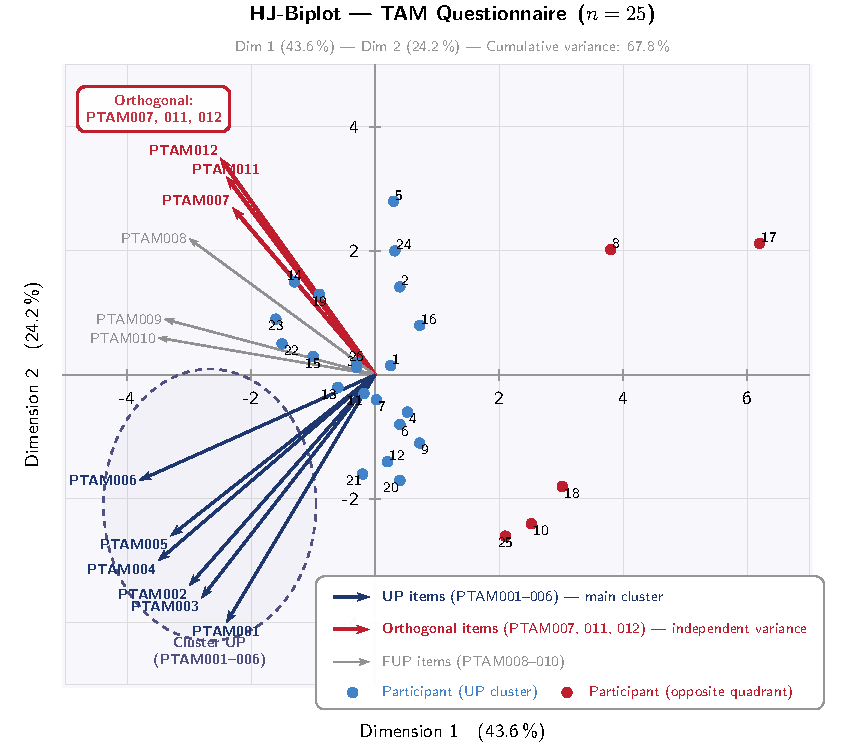
\includegraphics[width=\columnwidth]{biplot.pdf}
		\caption{HJ-Biplot of TAM questionnaire responses ($n=25$).
			Dimension~1 explains 43.6\,\% of variance; Dimension~2 explains 24.2\,\% (cumulative: 67.8\,\%). Arrows indicate item vectors;
			proximity of participant points to a vector reflects agreement with that item. The UP cluster (PTAM001--006) and most FUP items (PTAM008--010) point in the same direction, indicating high
			internal correlation. PTAM007 and PTAM012 are orthogonal to the main cluster, capturing independent variance.}
		\label{fig:biplot}
	\end{figure}
	
	\subsubsection{Observaci\'on Directa}
	La sesi\'on de observaci\'on directa registr\'o los indicadores conductuales definidos en el protocolo de evaluaci\'on: 7~errores de interacci\'on (toques en elementos incorrectos), 2~solicitudes de ayuda al facilitador y 15~toques err\'oneos totales. Los tres indicadores se concentraron mayoritariamente en la pantalla de mensajer\'ia y en la pantalla de c\'amara durante las tareas T2 y T4, en concordancia con la mayor densidad de elementos interactivos en esas pantallas y con el n\'umero residual de advertencias de accesibilidad documentado en la Tabla~\ref{tab:accesibilidad}. El bajo n\'umero de solicitudes de ayuda (2 sobre 25 participantes, 8\,\%) confirma que la mayor\'ia de los usuarios complet\'o las tareas predefinidas de forma aut\'onoma, en coherencia con las valoraciones positivas de UP.
	
	% ---------------------------------------------------------------
	\subsection{S\'intesis de Resultados}
	% ---------------------------------------------------------------
	La Tabla~\ref{tab:sintesis} ofrece una visi\'on integrada de los resultados obtenidos en las tres dimensiones evaluadas, relacionando cada resultado con la brecha identificada en la secci\'on~\ref{sec:relacionados} que aborda.
	
	\begin{table}[!t]
		\caption{S\'intesis de resultados por dimensi\'on de evaluaci\'on y brecha atendida.}
		\label{tab:sintesis}
		\centering
		%\small
		\renewcommand{\arraystretch}{1.25}
		\begin{tabular}{p{2.0cm}p{2.8cm}p{2.5cm}}
			\toprule
			\textbf{Dimensi\'on} & \textbf{Resultado principal} & \textbf{Brecha atendida} \\
			\midrule
			Rendimiento API   & Tasa de error~$=0$ en TTS, STT, \textit{captioning} y v\'ideo; latencia TTS m\'inima: 5.14~s; \textit{overhead} base64 en v\'ideo: ${\approx}40\%$ & Brechas~1 y~2 \\
			Accesibilidad    & Reducci\'on del 64\,\% en advertencias WCAG~2.1 (48/75); 100\,\% en c\'amara y foto & Brecha~4 \\
			Aceptaci\'on TAM & $\bar{x}_{global}=4.20$; UP~$=4.55$; FUP~$=3.85$ & Brecha~3 \\
			Observaci\'on    & 8\,\% solicitudes de ayuda; errores concentrados en mensajer\'ia & Brechas~1 y~5 \\
			\bottomrule
		\end{tabular}
	\end{table}
	
	% ---------------------------------------------------------------
	% VI. DISCUSION
	% ---------------------------------------------------------------
	\section{Discusi\'on}
	\label{sec:discusion}
	Esta secci\'on interpreta los resultados obtenidos en el marco de la literatura revisada, articula las implicaciones de los hallazgos para el campo de la interacci\'on hombre-m\'aquina inclusiva, identifica las limitaciones del sistema y reflexiona sobre el alcance social del trabajo.
	
	% ---------------------------------------------------------------
	\subsection{Interpretaci\'on de los Resultados T\'ecnicos}
	% ---------------------------------------------------------------
	Los cuatro m\'odulos de conversi\'on del sistema ---TTS, STT, descripci\'on de im\'agenes y procesamiento de v\'ideo--- operaron con tasa de error cero en todas las condiciones evaluadas, lo que valida la estabilidad de la arquitectura de microservicios propuesta y satisface el criterio de aceptaci\'on definido en la Fase~5 de TDDM4IoTS. Este resultado es relevante porque ninguno de los sistemas de mensajer\'ia inclusiva revisados en la literatura ---BellChat \cite{guerrero2021bellchat}, el prototipo de Stefanov~\textit{et al.} \cite{stefanov2024} ni GlassMessaging \cite{janaka2023}--- reporta evaluaciones de robustez API con condiciones de entrada variable, lo que impide la comparaci\'on directa de tasas de error pero resalta la contribuci\'on metodol\'ogica de disponer de evidencia cuantificada bajo un protocolo controlado.
	
	La latencia TTS m\'inima observada fue 5.14~s (SAPI5, texto corto), valor que excede el umbral de 2~s que Tan~\textit{et al.} \cite{tan2021} identifican como \'optimo para mantener el flujo conversacional en sistemas TTS neuronales de alta calidad. Esta limitaci\'on no es exclusiva del sistema propuesto: la revisi\'on PRISMA de Bercaru y Popescu \cite{bercaru2024} documenta que la latencia de inferencia sigue siendo la barrera de despliegue m\'as cr\'itica de los modelos TTS neuronales en entornos de producci\'on real, y que solo las implementaciones con cach\'e predictiva o modelos no autorregresivos logran latencias inferiores a 2~s. La ventaja de SAPI5 sobre Edge-TTS en latencia neta (37\,\% menor para texto corto) se explica por la ausencia de latencia de red en el procesamiento local; no obstante, este beneficio se revierte en escenarios con ancho de banda m\'ovil limitado, donde los archivos de respuesta de SAPI5 ---7.24~MB para texto largo frente a 0.75~MB de Edge-TTS--- representan una penalizaci\'on de transferencia significativa. Este \textit{trade-off} entre latencia de inferencia y volumen de datos de respuesta no hab\'ia sido documentado en el contexto de sistemas de mensajer\'ia inclusiva m\'ovil y constituye un hallazgo operacionalmente relevante para futuras implementaciones.
	
	La latencia del m\'odulo STT escal\'o de 13.36~s para audio corto a 54.99~s para audio largo, con integridad de transmisi\'on perfecta en todos los casos (diferencia entre env\'io y respuesta inferior al 1\,\%). Este comportamiento es coherente con la arquitectura de Whisper \cite{radford2023}, cuyo mecanismo de atenci\'on global sobre la secuencia completa de audio determina que el coste computacional sea proporcional a la duraci\'on. Baevski~\textit{et al.} \cite{baevski2020} demuestran que los modelos STT basados en aprendizaje autosupervisado ---como wav2vec~2.0, al que Whisper es conceptualmente cercano--- alcanzan WER comparable a la transcripci\'on humana, pero sus latencias de inferencia en producci\'on var\'ian notablemente seg\'un el hardware de despliegue. El nodo AWS utilizado represent\'o la soluci\'on m\'inima viable dada la infraestructura disponible; la reducci\'on de latencia STT mediante aceleraci\'on GPU dedicada o modelos destilados (\textit{Whisper Tiny/Small}) constituye la l\'inea de mejora de mayor impacto pr\'actico identificada.
	
	La variabilidad no mon\'otona observada en la latencia del m\'odulo de descripci\'on de im\'agenes ---la resoluci\'on 1\,920$\times$1\,280~px registr\'o menor latencia (16.42~s) que la resoluci\'on 1\,280$\times$853~px (17.67~s)--- es consistente con los hallazgos de Dognin~\textit{et al.} \cite{dognin2021}, quienes documentan que en el conjunto VizWiz la dificultad sem\'antica de la imagen ---no su resoluci\'on--- es el predictor primario del tiempo de inferencia en modelos de \textit{image captioning} basados en atenci\'on visual. Safiya y Pandian \cite{safiya2024} corroboran esta observaci\'on al reportar que el modelo VGG16-LSTM exhibe tiempos de inferencia variables en im\'agenes con alta densidad de objetos, independientemente de su tama\~no en p\'ixeles. Estos resultados tienen implicaciones de dise\~no: en una aplicaci\'on m\'ovil de mensajer\'ia inclusiva, la predicci\'on de latencia de descripci\'on no puede basarse exclusivamente en metadatos de tama\~no de imagen, sino que requiere un estimador de complejidad sem\'antica que anticipe los tiempos de respuesta para gestionar las expectativas del usuario.
	
	Un hallazgo operacionalmente relevante del m\'odulo de v\'ideo es el \textit{overhead} de transmisi\'on atribuible a la codificaci\'on base64 requerida por el protocolo HTTP \textit{multipart/form-data}: los tama\~nos de transmisi\'on efectivos (12.89~MB, 68.45~MB y 107.55~MB) superan en aproximadamente un 40\,\% los pesos originales de los archivos (9.22~MB, 48.9~MB y 76.9~MB). Este incremento debe considerarse en el dimensionamiento del ancho de banda y en las notificaciones de progreso al usuario durante la transferencia. La diferencia entre tama\~no de env\'io y respuesta fue inferior al 0.2\,\% en todos los casos, confirmando la integridad de la transmisi\'on independientemente del \textit{overhead} de codificaci\'on.
	
	% ---------------------------------------------------------------
	\subsection{Interpretaci\'on de los Resultados de Accesibilidad}
	% ---------------------------------------------------------------
	La reducci\'on global del 64.0\,\% en advertencias de accesibilidad (de 75 a 27) tras la aplicaci\'on del ciclo iterativo de TDDM4IoTS coloca al sistema propuesto en una posici\'on notablemente superior respecto a las plataformas comerciales de referencia. Chen~\textit{et al.} \cite{chen2022} documentan tasas de incumplimiento superiores al 60\,\% en criterios WCAG~2.1 fundamentales para WhatsApp, Telegram, Messenger e Instagram, valores que representan el escenario \textit{baseline} con el que el sistema propuesto compite. Huang~\textit{et al.} \cite{huang2025} confirman que estos patrones de incumplimiento son especialmente severos en los criterios de tama\~no de objetivo t\'actil y contraste de color para usuarios con discapacidades cognitivas, precisamente las dos categor\'ias m\'as frecuentes entre las 48 advertencias resueltas en el proceso iterativo de este trabajo.
	
	La reducci\'on del 100\,\% en las pantallas de c\'amara y foto valida que la metodolog\'ia de desarrollo adoptada ---en particular, la Fase~5 de TDDM4IoTS que define las pruebas de accesibilidad antes de la generaci\'on del c\'odigo--- es efectiva para eliminar barreras en pantallas de dise\~no relativamente simple. Este resultado concuerda con la propuesta de Ara~\textit{et al.} \cite{ara2024} de que el \textit{testing} iterativo desde fases tempranas del ciclo de desarrollo es la intervenci\'on con mayor impacto en la conformidad WCAG. Por el contrario, la pantalla de mensajer\'ia ---la de mayor densidad funcional del sistema--- s\'olo alcanz\'o una reducci\'on del 38.1\,\%, lo que expone una limitaci\'on arquitect\'onica del patr\'on de lista virtualizada de React Native que genera identificadores de accesibilidad duplicados. Esta limitaci\'on no es exclusiva del sistema propuesto: Da~Silva~\textit{et al.} \cite{dasilva2016} identificaron que las pantallas de conversaci\'on de WhatsApp concentran el mayor n\'umero de barreras para usuarios con discapacidad visual, y Swati~\textit{et al.} \cite{swati2021} documentaron el mismo patr\'on en Facebook Messenger. El problema es, por tanto, estructural al paradigma de lista de mensajes virtualizada y no resuelto en ninguna implementaci\'on reportada en la literatura.
	
	La evaluaci\'on de accesibilidad fue realizada exclusivamente con herramientas automatizadas (\textit{Accessibility Scanner}), en concordancia con la metodolog\'ia de Acosta-Vargas~\textit{et al.} \cite{acosta2021}, quienes demuestran que los m\'etodos automatizados detectan el espectro de barreras de tipo estructural con alta cobertura. Sin embargo, los propios autores advierten que el enfoque combinado ---automatizado m\'as inspecci\'on manual experta--- incrementa la cobertura de detecci\'on en m\'as de un 35\,\%. La ausencia de inspecci\'on manual experta en el presente estudio constituye, por tanto, una limitaci\'on metodol\'ogica reconocida que puede haber subestimado el n\'umero real de barreras presentes, especialmente en las dimensiones de comprensibilidad y robustez, cuya evaluaci\'on autom\'atica es parcial incluso en las herramientas m\'as avanzadas \cite{ara2024}.
	
	% ---------------------------------------------------------------
	\subsection{Interpretaci\'on de los Resultados de Aceptaci\'on Tecnol\'ogica}
	% ---------------------------------------------------------------
	La media global del cuestionario TAM ($\bar{x}=4.20$; DE~$=0.95$) supera el umbral de aceptaci\'on positiva $\bar{x} > 4.0$ establecido en estudios TAM en contextos de accesibilidad m\'ovil \cite{julianto2023}, lo que constituye evidencia de que los usuarios de la muestra perciben el sistema como una alternativa tecnol\'ogicamente aceptable a las plataformas convencionales. La solidez psicom\'etrica del instrumento queda confirmada por los coeficientes alfa de Cronbach ($\alpha_{global}=0.866$; $\alpha_{UP}=0.867$; $\alpha_{FUP}=0.898$), que superan el umbral de 0.80 considerado indicativo de buena consistencia interna \cite{nunnally1978}. Este resultado respalda directamente el paradigma de Davis \cite{davis1989}, que postula que la utilidad percibida es el predictor dominante de la adopci\'on, y es coherente con el patr\'on documentado por Mateos-Sanchez~\textit{et al.} \cite{mateos2022} en CapacitaBOT, donde las funcionalidades de conversi\'on con IA fueron las mejor valoradas.
	
	El constructo UP obtuvo la media m\'as alta ($\bar{x}_{UP}=4.55$), con PTAM002 como el \'item mejor valorado ($\bar{x}=4.76$; 84\,\% en nivel~5). Este resultado indica que la eficacia comunicativa mediada por el sistema es la aportaci\'on de mayor valor pr\'actico, lo que valida el argumento de Elsahar~\textit{et al.} \cite{elsahar2019} de que la velocidad conversacional ---no la precisi\'on de la conversi\'on--- es el factor cr\'itico de usabilidad en plataformas CAA. Los \'items PTAM005 ($\bar{x}=4.56$) y PTAM006 ($\bar{x}=4.52$), integrados en UP seg\'un el instrumento utilizado, confirman adicionalmente que las interacciones y conversaciones facilitadas por el sistema responden a necesidades comunicativas reales, en l\'inea con Chang~\textit{et al.} \cite{chang2022}.
	
	El constructo FUP present\'o mayor dispersi\'on interna ($\bar{x}_{FUP}=3.85$). PTAM007 ($\bar{x}=3.56$; DE~$=1.36$) obtuvo la valoraci\'on m\'as baja del instrumento, con variabilidad en el rango completo 1--5. Este resultado resuena con los hallazgos de Bleakley~\textit{et al.} \cite{bleakley2022}: los sistemas de reconocimiento de voz comerciales presentan barreras para usuarios con baja experiencia tecnol\'ogica ---el 40\,\% de la muestra--- relacionadas con la curva de aprendizaje de paradigmas de interacci\'on por voz. PTAM012 ($\bar{x}=3.48$) y PTAM011 ($\bar{x}=3.72$), con el 20\,\% y el 28\,\% de participantes en el nivel~1 respectivamente, indican que el dominio completo de todas las funciones requiere un proceso de apropiaci\'on m\'as extendido que el protocolo de evaluaci\'on de 20~minutos. El fen\'omeno de ``expectativas elevadas en poblaciones con alta dependencia de herramientas de accesibilidad'', documentado por Weichbroth \cite{weichbroth2020}, es la interpretaci\'on m\'as coherente con la baja puntuaci\'on en los \'items de f\'acil uso percibido.
	
	El an\'alisis HJ-Biplot (Figura~\ref{fig:biplot}) evidenci\'o que los vectores de PTAM007 y PTAM012 son ortogonales al cl\'uster principal formado por los restantes \'items, capturando varianza independiente asociada a la apropiaci\'on de la interacci\'on por voz y el dominio funcional completo. Este patr\'on es te\'oricamente consistente con el TAM original \cite{davis1989}, en el que la facilidad de uso modera el efecto de la utilidad percibida sobre la intenci\'on de adopci\'on, y ha sido documentado en aplicaciones CAA por Kim~\textit{et al.} \cite{kim2024}.
	
	% ---------------------------------------------------------------
	\subsection{Implicaciones para el Dise\~no de Sistemas de Mensajer\'ia Inclusiva}
	% ---------------------------------------------------------------
	Los resultados del presente estudio permiten articular cuatro implicaciones concretas para el dise\~no de sistemas de mensajer\'ia inclusiva impulsados por IA.
	
	La primera implicaci\'on es que la \textbf{integraci\'on multimodal} de TTS, STT, \textit{image captioning} y OCR en una plataforma m\'ovil \'unica es t\'ecnicamente viable con tecnolog\'ias de c\'odigo abierto disponibles, y produce niveles de aceptaci\'on tecnol\'ogica positivos ($\bar{x}_{TAM}=4.20$; $\bar{x}_{UP}=4.55$; $\bar{x}_{FUP}=3.85$) en poblaciones con discapacidad sensorial heterog\'enea. Este hallazgo no ten\'ia precedente documentado en la literatura, que se hab\'ia limitado a sistemas unimodales \cite{guerrero2021bellchat} o de perfil \'unico \cite{stefanov2024, yeratziotis2023}.
	
	La segunda implicaci\'on es que el \textbf{cifrado asim\'etrico de extremo a extremo} es compatible con el flujo de conversi\'on multimodal sin degradar la tasa de error, lo que disipa la preocupaci\'on --impl\'icita en la brecha identificada--- de que la privacidad y la accesibilidad son objetivos en conflicto en sistemas de mensajer\'ia. Ninguno de los sistemas CAA revisados ---incluyendo Talkitt \cite{costanzo2023}, CapacitaBOT \cite{mateos2022} y BellChat \cite{guerrero2021bellchat}--- hab\'ia reportado una implementaci\'on de privacidad equivalente.
	
	La tercera implicaci\'on es que el \textbf{m\'odulo de comandos de voz} mediante similitud del coseno con correci\'on en cascada reduce, pero no elimina, la barrera de la curva de aprendizaje para la navegaci\'on por voz (PTAM007: $\bar{x}=3.56$). El dise\~no de un proceso de \textit{onboarding} accesible que guíe al usuario en la internalizaci\'on de los comandos disponibles es una condici\'on necesaria para que el sistema alcance su potencial de accesibilidad plena para usuarios con discapacidad visual severa.
	
	La cuarta implicaci\'on concierne a la \textbf{metodolog\'ia de desarrollo}. La aplicaci\'on de TDDM4IoTS \cite{guerrero2020} con accesibilidad como criterio verificable desde la Fase~5 produjo una reducci\'on del 64\,\% en advertencias WCAG~2.1, resultado que contrasta con la ausencia total de evaluaci\'on de accesibilidad en los ciclos de desarrollo de los sistemas CAA revisados \cite{costanzo2023, mateos2022, janaka2023}. Este dato sugiere que la incorporaci\'on de pruebas de accesibilidad como requisito de aceptaci\'on ---en lugar de actividades \textit{post-hoc}--- es la intervenci\'on de mayor impacto en la calidad de accesibilidad del artefacto final, en consonancia con la recomendaci\'on central de Ara~\textit{et al.} \cite{ara2024}.
	
	% ---------------------------------------------------------------
	\subsection{Limitaciones del Estudio y Trabajo Futuro}
	% ---------------------------------------------------------------
	El presente estudio presenta cuatro limitaciones que deben tenerse en cuenta al interpretar sus resultados.
	
	La primera es el \textbf{tama\~no muestral}: $n=25$ participantes, si bien justificado por la especificidad cl\'inica de los criterios de inclusi\'on y el car\'acter proyectivo de la investigaci\'on \cite{hernandez2014}, no permite generalizar los resultados a la diversidad de perfiles de discapacidad sensorial ni a otros contextos geogr\'aficos y culturales. La ampliaci\'on del estudio con muestras estratificadas por tipo de discapacidad y rango de edad es la l\'inea de trabajo futuro de mayor prioridad para incrementar la generalizabilidad de los hallazgos.
	
	La segunda limitaci\'on es la \textbf{latencia TTS}: con valores m\'inimos de 5.14~s, el sistema no alcanza a\'un el umbral conversacional de 2~s \cite{tan2021}. La optimizaci\'on mediante modelos TTS no autorregresivos (FastSpeech2, VITS) ejecutados localmente en el dispositivo m\'ovil, o mediante cach\'e predictiva de segmentos de voz frecuentes, es la mejora t\'ecnica de mayor impacto identificada.
	
	La tercera limitaci\'on es la \textbf{pantalla de mensajer\'ia con accesibilidad residual} (38.1\,\% de reducci\'on vs. 100\,\% en otras pantallas), cuya causa es arquitect\'onica: el patr\'on de lista virtualizada en React Native genera identificadores de accesibilidad duplicados que ning\'un ciclo de mejora puede resolver sin refactorizar la arquitectura de identificadores \'unicos din\'amicos por elemento.
	
	La cuarta limitaci\'on es la \textbf{ausencia de reconocimiento de lenguaje de se\~nas}, lo que excluye a usuarios sordos cuya lengua materna no es el espa\~nol escrito sino la lengua de se\~nas. La integraci\'on de un m\'odulo RALS ---como los propuestos por Saleem~\textit{et al.} \cite{saleem2023} y Kothadiya~\textit{et al.} \cite{kothadiya2022}--- es la extensi\'on funcional m\'as significativa para ampliar la cobertura del sistema a este colectivo.
	
	% ---------------------------------------------------------------
	\subsection{Alineaci\'on con los Objetivos de Desarrollo Sostenible}
	% ---------------------------------------------------------------
	Los resultados del presente trabajo se alinean con dos Objetivos de Desarrollo Sostenible (ODS) de la Agenda~2030 de las Naciones Unidas. En relaci\'on con el ODS~10 (Reducci\'on de las Desigualdades), el sistema demuestra que la tecnolog\'ia m\'ovil con IA puede reducir las asimetr\'ias comunicativas que marginan a 124{,}801 personas con discapacidades sensoriales en Ecuador ---cifra que la OMS escala al 15\,\% de la poblaci\'on mundial \cite{who2011}--- de la comunicaci\'on digital aut\'onoma. En relaci\'on con el ODS~9 (Industria, Innovaci\'on e Infraestructura), el sistema propone una arquitectura de microservicios desplegable sobre infraestructura h\'ibrida de bajo coste (servidor institucional m\'as instancia en nube), lo que reduce la barrera de adopci\'on institucional en contextos de recursos limitados como el de la UTEQ. La compatibilidad entre accesibilidad, privacidad e infraestructura asequible que demuestra el sistema constituye un modelo de referencia transferible a otros contextos de inclusi\'on digital en pa\'ises en desarrollo.
	
	% ---------------------------------------------------------------
	% VII. CONCLUSI\'ON
	% ---------------------------------------------------------------
	\section{Conclusi\'on}
	\label{sec:conclusion}
	Este art\'iculo ha presentado el dise\~no, implementaci\'on y evaluaci\'on emp\'irica de un sistema de mensajer\'ia m\'ovil inclusiva potenciado por inteligencia artificial, concebido para atender los perfiles sensoriales visual y auditivo mediante la orquestaci\'on integrada de m\'odulos TTS, STT, descripci\'on autom\'atica de im\'agenes y OCR, con cifrado asim\'etrico de extremo a extremo y navegaci\'on completa por comandos de voz. Los hallazgos permiten formular cuatro conclusiones sustantivas y cinco l\'ineas de investigaci\'on futura que avanzan el estado del arte en interacci\'on hombre-m\'aquina inclusiva.
	
	La \textbf{primera conclusi\'on} concierne a la viabilidad t\'ecnica de la integraci\'on multimodal con privacidad garantizada. Los cuatro m\'odulos de conversi\'on ---TTS, STT, \textit{image captioning} y v\'ideo--- registraron tasa de error cero en la totalidad de las condiciones de prueba, con integridad de transmisi\'on verificada en cada condici\'on (diferencia entre tama\~no de env\'io y respuesta inferior al 1\,\% en STT y al 0.2\,\% en v\'ideo). La coexistencia del flujo de conversi\'on accesible con el cifrado asim\'etrico de extremo a extremo, sin degradar la tasa de error, demuestra por primera vez en la literatura de mensajer\'ia inclusiva que la privacidad y la accesibilidad no son objetivos en conflicto en una arquitectura m\'ovil distribuida. La latencia TTS m\'inima de 5.14~s (SAPI5, texto corto) constituye la limitaci\'on t\'ecnica principal al superar el umbral conversacional de 2~s; su resoluci\'on mediante modelos TTS no autorregresivos o cach\'e predictiva de segmentos representa la mejora de mayor urgencia para versiones futuras del sistema.
	
	La \textbf{segunda conclusi\'on} concierne a la aceptaci\'on tecnol\'ogica positiva en una poblaci\'on de discapacidad heterog\'enea. El cuestionario TAM de 12~\'items ---organizado en sus dos constructos cl\'asicos UP y FUP \cite{davis1989}--- aplicado a $n=25$ participantes (60\,\% con discapacidad visual, 20\,\% auditiva, 20\,\% sin discapacidad) produjo una media global de $\bar{x}=4.20$ (DE~$=0.95$), que supera el umbral de aceptaci\'on positiva $\bar{x}>4.0$ \cite{julianto2023}. La consistencia interna del instrumento fue s\'olida: $\alpha_{global}=0.866$, $\alpha_{UP}=0.867$ y $\alpha_{FUP}=0.898$, todos superiores al umbral de 0.80 \cite{nunnally1978}. El constructo UP alcanz\'o $\bar{x}_{UP}=4.55$, con PTAM002 ($\bar{x}=4.76$; 84\,\% en nivel~5) como la aportaci\'on de mayor valor pr\'actico percibida. La curva de aprendizaje inicial de la navegaci\'on por voz (PTAM007: $\bar{x}=3.56$; DE~$=1.36$) y el dominio completo de funciones (PTAM012: $\bar{x}=3.48$) representan las dos dimensiones de mejora prioritarias del constructo FUP ($\bar{x}_{FUP}=3.85$). El bajo n\'umero de solicitudes de ayuda (2 de 25 participantes, 8\,\%) confirma que la mayor\'ia de los usuarios complet\'o las tareas predefinidas de forma aut\'onoma.
	
	La \textbf{tercera conclusi\'on} concierne a la eficacia del ciclo iterativo de TDDM4IoTS para la mejora sistem\'atica de la accesibilidad. La aplicaci\'on de la metodolog\'ia \cite{guerrero2020} con la accesibilidad como criterio de aceptaci\'on verificable desde la Fase~5 ---anterior a la generaci\'on del c\'odigo--- produjo una reducci\'on global del 64.0\,\% en advertencias WCAG~2.1 (de 75 a 27), con eliminaci\'on total en las pantallas de c\'amara y foto (100\,\%) y reducciones superiores al 70\,\% en configuraciones (77.8\,\%) y pantalla principal (81.8\,\%). Este resultado contrasta con las tasas de incumplimiento superiores al 60\,\% documentadas en las plataformas de mensajer\'ia comerciales de referencia \cite{chen2022} y valida que la incorporaci\'on de pruebas de accesibilidad como requisito formal de aceptaci\'on ---en lugar de actividades \textit{post-hoc}--- es la intervenci\'on de mayor impacto en la calidad de accesibilidad del artefacto. La limitaci\'on residual en la pantalla de mensajer\'ia (38.1\,\%) responde a una causa arquitect\'onica identificada ---identificadores de accesibilidad duplicados generados por el patr\'on de lista virtualizada de React Native--- con protocolo de resoluci\'on definido, lo que la convierte en una deuda t\'ecnica trazable.
	
	La \textbf{cuarta conclusi\'on} concierne a la resoluci\'on de la fragmentaci\'on tecnol\'ogica documentada en la literatura. Los componentes de IA para la accesibilidad ---TTS neuronal, STT basado en transformadores, \textit{image captioning} y OCR--- que la literatura ha desarrollado de forma aislada \cite{tan2021, baevski2020, radford2023, ming2022, mukherjee2023} son integrables en una arquitectura de mensajer\'ia m\'ovil coherente, estable y con privacidad garantizada mediante infraestructura h\'ibrida de bajo coste institucional. Esta integraci\'on, ausente en todos los sistemas revisados, establece un modelo de referencia transferible para el desarrollo de aplicaciones de comunicaci\'on inclusiva en contextos con restricciones de infraestructura, con implicaciones directas para el cumplimiento del ODS~10 (Reducci\'on de Desigualdades) y el ODS~9 (Industria, Innovaci\'on e Infraestructura) de la Agenda~2030 de las Naciones Unidas.
	
	Los hallazgos configuran cinco l\'ineas de investigaci\'on futura de alta prioridad. La primera es la optimizaci\'on de la latencia TTS mediante arquitecturas no autorregresivas ---FastSpeech2 o VITS--- ejecutadas localmente en el dispositivo m\'ovil, o mediante cach\'e predictiva de segmentos de voz basada en patrones de mensajer\'ia frecuentes, con el objetivo de alcanzar el umbral conversacional de 2~s establecido en la literatura \cite{tan2021}. La segunda es el dise\~no de un flujo de \textit{onboarding} accesible que incluya calibraci\'on personalizada de comandos de voz al perfil de disfluencia del usuario, siguiendo el paradigma de entrenamiento adaptativo de Costanzo~\textit{et al.} \cite{costanzo2023}, para reducir la barrera de aprendizaje documentada en PTAM007. La tercera es la integraci\'on de reconocimiento de lenguaje de se\~nas como modalidad adicional de entrada y salida, tomando como referentes los modelos LSTM--GRU de Kothadiya~\textit{et al.} \cite{kothadiya2022} y los sistemas multiling\"ues de Saleem~\textit{et al.} \cite{saleem2023}. La cuarta es la refactorizaci\'on arquitect\'onica de la pantalla de mensajer\'ia mediante identificadores de accesibilidad \'unicos din\'amicos por elemento de lista, con el objetivo de eliminar las 13 advertencias residuales y elevar la satisfacci\'on global del sistema (PTAM012: $\bar{x}=3.48$). La quinta es la ampliaci\'on del estudio a muestras estratificadas por tipo de discapacidad, rango de edad y condiciones de conectividad m\'ovil (redes 4G/LTE de bajo ancho de banda), para incrementar la generalizabilidad de los resultados e identificar factores de moderaci\'on de la aceptaci\'on tecnol\'ogica espec\'ificos a cada perfil sensorial.
	
	% ---------------------------------------------------------------
	% AGRADECIMIENTOS
	% ---------------------------------------------------------------
	\section*{Agradecimientos}
	Los autores agradecen a la Universidad T\'ecnica Estatal de Quevedo (UTEQ) por el apoyo t\'ecnico, financiero e institucional. De igual forma, expresan su gratitud a los 25 participantes del estudio, cuya colaboraci\'on fue fundamental para la validaci\'on emp\'irica del sistema propuesto.

	% ---------------------------------------------------------------
	\bibliographystyle{IEEEtran}
	\bibliography{refs}
	
\end{document}